\documentclass[12pt]{article}
\usepackage[utf8]{inputenc}
\usepackage{color,soul,CJK,epic,tikz,array}
\usepackage{amsmath,amsthm,amssymb}
\setlength{\parindent}{0em}

\theoremstyle{definition}
\newtheorem{definition}{Definition}[section]
\newtheorem{theorem}[definition]{Theorem}
\newtheorem{remark}[definition]{Remark}
\newtheorem{lemma}[definition]{Lemma}
\newtheorem{corollary}[definition]{Corollary}
\newtheorem{example}[definition]{Example}

\newcommand\<{\langle}
\renewcommand\>{\rangle}
\newcommand\obj{\mathrm{obj}\hspace{2pt}}
\newcommand\im{\mathrm{im}\hspace{2pt}}
\newcommand\rel{\ \mathrm{rel}\ }
\newcommand\diam{\mathrm{diam}\hspace{2pt}}

\begin{document}
\begin{CJK}{UTF8}{bsmi}

\title{Topology}
\author{AndersonWu2000}
\maketitle

\section{Introduction}

\begin{definition}
    令 $X$ 為集合。函數 $1_X:X\to X:x\mapsto x$ 稱為 $X$ 的恆等函數 (identity)。
\end{definition}

\begin{remark}
    令 $f:X\to Y$ 為一個函數,$\{X_\alpha\ |\ \alpha\in A\}\subseteq\mathcal{P}(X)$ 和 $\{Y_\alpha\ |\ \alpha\in A\}\subseteq\mathcal{P}(Y)$ 為集族:
    \begin{enumerate}
        \item $f(\bigcap_{\alpha\in A} X_\alpha)\subseteq\bigcap_{\alpha\in A}f(X_\alpha)$。
        \item $f(\bigcup_{\alpha\in A} X_\alpha)=\bigcup_{\alpha\in A}f(X_\alpha)$。
        \item $f^{-1}(\bigcap_{\alpha\in A} Y_\alpha)=\bigcap_{\alpha\in A}f^{-1}(Y_\alpha)$。
        \item $f^{-1}(\bigcup_{\alpha\in A} Y_\alpha)=\bigcup_{\alpha\in A}f^{-1}(Y_\alpha)$。
    \end{enumerate}
\end{remark}

\begin{definition}
    令 $X_1, \cdots, X_n$ 為集合。對於 $1\le i\le n$,函數 
    \[
        \pi_i:\prod_{i=1}^n X_i\to X_i:(x_1, \cdots, x_n)\mapsto x_i
    \]
    稱為投影函數 (projection)。
\end{definition}

\begin{remark}
\label{property of cartesian product}
    令 $A, B, C, D$ 為集合:
    \begin{enumerate}
        \item $A\times\varnothing=\varnothing$。
        \item $(A\times B)\cap(A\times C)=A\times(B\cap C)$。
        \item $(A\times B)\cup(A\times C)=A\times(B\cup C)$。
        \item $(A\times B)\cap(C\times D)=(A\cap C)\times(B\cap D)$。
        \item $(A\times B)\cup(C\times D)\subseteq(A\cup C)\times(B\cup D)$。
    \end{enumerate}
\end{remark}

\begin{definition}
    令 $x=(x_1, \cdots, x_n)\in\mathbb{R}^n$,定義 $x$ 的範數 (norm) 為 
    \[
        \|x\|=\sqrt{\sum_{i=1}^n x_i^2}.
    \]
\end{definition}

\begin{definition}
    $\{x\in\mathbb{R}^{n+1}\ |\ \|x\|=1\}$ 稱為 $n$-球面 (sphere),記為 $S^n$。$\{x\in\mathbb{R}^{n+1}\ |\ \|x\|\le1\}$ 稱為 $n$-球 (ball),記為 $D^n$。
\end{definition}

$\mathbb{R}^{n}$ 上的標準基記為 $e_0, \cdots, e_{n-1}$。

$[0, 1]$ 記為 $\textbf{I}$。

\begin{definition}
    令 $X$ 為集合。由所有 $X$ 上的對射 $f:X\to X$ 在複合運算下組成的群稱為對稱群 (symmetric group),其子群稱為置換群 (permutation group)。
\end{definition}

\begin{definition}
    令 $F$ 為群,$B$ 為 $F$ 的子集。若對於所有群 $G$ 和函數 $\phi:B\to G$,存在唯一的同態 $\hat{\phi}:F\to G$ 使得 $\hat{\phi}|_B=\phi$,則稱 $F$ 為由 $B$ 生成的自由群 (free group),稱 $B$ 為 $F$ 的基 (basis)。
\end{definition}

\begin{definition}
    令 $F$ 為交換群,$B$ 為 $F$ 的子集。若對於所有交換群 $G$ 和函數 $\phi:B\to G$,存在唯一的同態 $\hat{\phi}:F\to G$ 使得 $\hat{\phi}|_B=\phi$,則稱 $F$ 為由 $B$ 生成的自由交換群 (free abelian group),稱 $B$ 為 $F$ 的基 (basis)。
\end{definition}

若 $F$ 為自由群且為自由交換群,則 $F\cong\{0\}$ 或 $F\cong\mathbb{Z}$。 \\

令 $(F, +)$ 為由 $B$ 生成的自由交換群,則所有 $b\in B$ 滿足 $\<b\>\cong\mathbb{Z}$ 且
\[
    F = \left\{\left.\sum_{i=1}^k n_i b_i\ \right|\ k\in\mathbb{N}, n_1, \cdots, n_k\in\mathbb{Z}, b_1, \cdots, b_k\in B\right\}
\]

\section{Category}

\begin{definition}
    令 $\obj\mathcal{C}$ 為物件的蒐集:
    \begin{enumerate}
        \item 對於所有 $A, B\in\obj\mathcal{C}$,令 $\hom(A, B)$ 為一個集合。
        \item 對於所有 $A, B, C\in\obj\mathcal{C}$,令 $\circ:\hom(A, B)\times\hom(B, C)\to\hom(A, C)$ 為一個二元算子,記為 $g\circ f$。
    \end{enumerate}
    令 $\hom\mathcal{C}$ 為 $\obj\mathcal{C}$ 上所有 $\hom(A, B)$ 的蒐集。若 $\mathcal{C}=(\obj\mathcal{C}, \hom\mathcal{C}, \circ)$ 滿足下列條件,則稱 $\mathcal{C}$ 為一個範疇 (category):
    \begin{enumerate}
        \item 令 $f\in\hom(A, B), g\in\hom(B, C), h\in\hom(C, D)$。
        \[
            h\circ(g\circ f)=(h\circ g)\circ f.
        \]
        \item 令 $A, B, X\in\obj\mathcal{C}$。存在 $1_X\in\hom(X, X)$ 使得所有 $f\in\hom(A, X), g\in\hom(X, B)$ 滿足 $1_X\circ f=f$ 和 $g\circ 1_X=g$。
    \end{enumerate}
\end{definition}

$\mathcal{C}=(\obj\mathcal{C}, \hom\mathcal{C}, \circ)$ 可以簡寫為 $\mathcal{C}=(\obj\mathcal{C}, \hom\mathcal{C})$。

\begin{definition}
    令 $\mathcal{C}=(\obj\mathcal{C}, \hom\mathcal{C}, \circ)$ 為一個範疇。二元算子 $\circ$ 稱為 $\mathcal{C}$ 的複合 (composition)。
\end{definition}

\begin{definition}
    令 $A, B$ 為 $\obj\mathcal{C}$ 的物件。$\hom(A, B)$ 內的元素 $f$ 稱為態射 (morphism),$A$ 稱為 $f$ 的域或源物件 (domain/source object),$B$ 稱為 $f$ 的對應域或目標物件 (codomain/target object),記為 $f:A\to B$。
\end{definition}

\begin{definition}
    集合範疇 $\textbf{Set}$ 定義如下:
    \begin{enumerate}
        \item 若 $A$ 為集合,則 $G\in\obj\textbf{Set}$。
        \item 若 $f:A\to B$ 為函數,則 $f\in\hom(A, B)$。
        \item 複合 $\circ$ 為函數複合。
    \end{enumerate}
\end{definition}

\begin{definition}
    群範疇 $\textbf{Grp}$ 定義如下:
    \begin{enumerate}
        \item 若 $G$ 為群,則 $G\in\obj\textbf{Grp}$。
        \item 若 $f:G\to H$ 為同態,則 $f\in\hom(G, H)$。
        \item 複合 $\circ$ 為函數複合。
    \end{enumerate}
\end{definition}

\begin{definition}
    阿貝爾群範疇 $\textbf{Ab}$ 定義如下:
    \begin{enumerate}
        \item 若 $G$ 為交換群,則 $G\in\obj\textbf{Ab}$。
        \item 若 $f:G\to H$ 為同態,則 $f\in\hom(G, H)$。
        \item 複合 $\circ$ 為函數複合。
    \end{enumerate}
\end{definition}

\begin{definition}
    令 $\mathcal{C}, \mathcal{D}$ 為範疇。若 $\mathcal{C}, \mathcal{D}$ 滿足下列條件,則稱 $\mathcal{C}$ 是 $\mathcal{D}$ 的子範疇 (subcategory):
    \begin{enumerate}
        \item $\obj\mathcal{C}\subseteq\obj\mathcal{D}$。
        \item 若 $A, B\in\obj\mathcal{C}$,則 $\hom_{\mathcal{C}}(A, B)\subseteq\hom_{\mathcal{D}}(A, B)$。
        \item 對於 $\mathcal{C}$ 的態射而言,$\mathcal{C}, \mathcal{D}$ 的複合相同。
    \end{enumerate}
\end{definition}

\begin{definition}
    令 $\mathcal{C}, \mathcal{D}$ 為範疇,$F$ 為一個函數。若 $F$ 滿足下列條件,則稱 $F$ 是從 $\mathcal{C}$ 到 $\mathcal{D}$ 的函子 (functor),記為 $F:\mathcal{C}\to\mathcal{D}$:
    \begin{enumerate}
        \item 若 $A\in\obj\mathcal{C}$,則 $F(A)\in\obj\mathcal{D}$。
        \item 若 $f:A\to B$ 是 $\mathcal{C}$ 的一個態射,則 $F(f):F(A)\to F(B)$ 是 $\mathcal{D}$ 的一個態射。
        \item 若 $f:A\to B, g:B\to C$ 是 $\mathcal{C}$ 的態射,則 $F(g\circ f)=F(g)\circ F(f)$。
        \item 若 $A\in\obj\mathcal{C}$,則 $F(1_A)=1_{F(A)}$。
    \end{enumerate}
\end{definition}

\begin{definition}
    令 $\mathcal{C}, \mathcal{D}$ 為範疇,$F$ 為一個函數。若 $F$ 滿足下列條件,則稱 $F$ 是從 $\mathcal{C}$ 到 $\mathcal{D}$ 的反變函子 (contravariant functor),記為 $F:\mathcal{C}\to\mathcal{D}$:
    \begin{enumerate}
        \item 若 $A\in\obj\mathcal{C}$,則 $F(A)\in\obj\mathcal{D}$。
        \item 若 $f:A\to B$ 是 $\mathcal{C}$ 的一個態射,則 $F(f):F(B)\to F(A)$ 是 $\mathcal{D}$ 的一個態射。
        \item 若 $f:A\to B, g:B\to C$ 是 $\mathcal{C}$ 的態射,則 $F(g\circ f)=F(f)\circ F(g)$。
        \item 若 $A\in\obj\mathcal{C}$,則 $F(1_A)=1_{F(A)}$。
    \end{enumerate}
\end{definition}

\begin{definition}
    圖表 (diagram) 是以物件為頂點,態射為邊的有向圖。 \\
    若圖表內任兩條起終點相同的路徑,在態射複合之下都相等,則稱該圖表為交換圖表或是可交換的 (commutative)。
\end{definition}

\section{Affine Space}

\begin{definition}
    令 $X$ 為 $\mathbb{R}^n$ 的子集。若對於所有 $x, y\in X$ 和 $t\in\textbf{I}$ 都有 $tx+(1-t)y\in X$,則稱 $X$ 是凸的 (convex)。
\end{definition}

\begin{definition}
    令 $X$ 為 $\mathbb{R}^n$ 的子集。若對於所有 $x, y\in X$ 和 $t\in\mathbb{R}$ 都有 $tx+(1-t)y\in X$,則稱 $X$ 是仿射的 (affine)。
\end{definition}

$tx+(1-t)y$ 是連接 $x, y$ 兩點的直線。

\begin{remark}
    令 $A$ 為仿射空間,$p$ 為 $A$ 內一點。$A-p_0$ 為向量空間。
\end{remark}
\begin{proof}
    Let $x_1=p_1-p, x_2=p_2-p\in A$ and $c\in\mathbb{R}$. \\
    If $c\ne-1$, then
    \[
        cx_1+x_2+p
         = (c+1)\left(\frac{c}{c+1}p_1+\frac{1}{c+1}p_2\right)-cp
         \in A.
    \]
    Otherwise,
    \[
        cx_1+x_2+p
         = (1-c)\left(\frac{-c}{1-c}p+\frac{1}{1-c}p_2\right)+cp_1
         \in A.
    \]
    Hence $A-p$ is a vector space.
\end{proof}

\begin{definition}
    令 $A$ 為仿射空間,$p$ 為 $A$ 內一點。$A$ 的維度 (dimension) 為 $\dim(A-p)$,記為 $\dim A$。
\end{definition}

\begin{definition}
    令 $p_0, p_1, \cdots, p_m\in\mathbb{R}^n$ 和 $t_0, t_1, \cdots, t_m\in\textbf{I}$。若 $\sum_{i=0}^m t_i=1$,則稱 $\sum_{i=0}^m t_i p_i$ 為凸組合 (convex combination)。
\end{definition}

換言之,凸組合涵蓋了以 $p_0, p_1, \cdots, p_m$ 為頂點,以連接頂點的直線為邊,其內部所圍成的凸集。

\begin{definition}
    令 $p_0, p_1, \cdots, p_m\in\mathbb{R}^n$ 和 $t_0, t_1, \cdots, t_m\in\mathbb{R}$。若 $\sum_{i=0}^m t_i=1$,則稱 $\sum_{i=0}^m t_i p_i$ 為仿射組合 (affine combination)。
\end{definition}

$\sum_{i=0}^m t_i p_i$ 可以寫為 $p_0+\sum_{i=1}^m t_i(p_i-p_0)$,$t_1, \cdots, t_m$ 即為任意實數。

換言之,仿射組合是位移後的線性組合。

\begin{definition}
    令 $p_0, \cdots, p_m\in\mathbb{R}^n$,則
    \[
        \left\{\sum_{i=0}^m t_i p_i\ \left|\ t_0, \cdots, t_m\in\textbf{I}, \sum_{i=0}^m t_i=1\right.\right\}
    \]
    稱為由 $p_0, \cdots, p_m$ 生成的凸集 (spanned),記為 $[p_0, \cdots, p_m]$;
    \[
        \left\{\sum_{i=0}^m t_i p_i\ \left|\ t_0, \cdots, t_m\in\mathbb{R}, \sum_{i=0}^m t_i=1\right.\right\}
    \]
    稱為由 $p_0, \cdots, p_m$ 生成的仿射集。
\end{definition}

\begin{definition}
    令 $p_0, \cdots, p_m\in\mathbb{R}^n$。若 $$\{p_1-p_i, \cdots, p_{i-1}-p_i, p_{i+1}-p_i, \cdots, p_m-p_i\}$$ 是線性獨立的,則稱 $\{p_0, \cdots, p_m\}$ 是仿射獨立的 (affine independent)。
\end{definition}

若 $\{p_1, \cdots, p_m\}$ 線性獨立,則 $\{0, p_1, \cdots, p_m\}$ 仿射獨立,但 $\{0, p_1, \cdots, p_m\}$ 不是線性獨立的。

\begin{corollary}
    令 $A$ 為仿射獨立集 $\{p_0, \cdots, p_m\}$ 生成的仿射集,$p$ 為 $A$ 內一點。存在唯一的 $t_0, \cdots, t_m\in\mathbb{R}$ 使得 $p=\sum_{i=0}^m t_i p_i$ 且 $1=\sum_{i=0}^m t_i$。
\end{corollary}
\begin{proof}
    Note that $A-p_0$ is a vector space. \\
    Since $A$ is generated by $\{p_0, \cdots, p_m\}$, there exists $t_0, \cdots, t_m\in\mathbb{R}$ such that $p=\sum_{i=0}^m t_i p_i$ and $1=\sum_{i=0}^m t_i$, so $p=p_0+\sum_{i=1}^m t_i(p_i-p_0)$. \\
    Then $p-p_0$ is a linear combination of $\{p_1-p_0, \cdots, p_m-p_0\}$. \\
    Since $\{p_1-p_0, \cdots, p_m-p_0\}$ is linearly independent, $\{t_1, \cdots, t_m\}$ is unique.
\end{proof}

令 $r_0, \cdots, r_m\in\mathbb{R}^n$。矩陣
\[
    V =
    \begin{bmatrix}
        r_0^0 & r_0^1 & \cdots & r_0^m \\
        r_1^0 & r_1^1 & \cdots & r_1^m \\
        \cdots \\
        r_m^0 & r_m^1 & \cdots & r_m^m 
    \end{bmatrix}
\]
稱為范德蒙矩陣 (Vandermonde matrix)。 \\

范德蒙矩陣 $V$ 的行列式為 $\det V=\prod_{j<i}(r_i-r_j)$。

若 $\{r_0, \cdots, r_m\}$ 沒有重複的元素,則 $V$ 是可逆的。

\begin{definition}
    令 $x_0, \cdots, x_m\in\mathbb{R}^n$。若 $\{x_0, \cdots, x_m\}$ 的任 $n+1$ 個元素是仿射獨立的,則稱 $\{x_0, \cdots, x_m\}$ 在一般位置 (general position)。
\end{definition}

\begin{theorem}
    令 $k$ 為自然數。存在 $x_0, \cdots, x_k\in\mathbb{R}^n$ 使得 $\{x_0, \cdots, x_m\}$ 在一般位置。
\end{theorem}
\begin{proof}
    It is trivial for $k\le n$. \\
    Otherwise, let $r_0, \cdots, r_k\in\mathbb{R}$ be distinct points. \\
    Define $x_i=(r_i^1, r_i^2, \cdots, r_i^n)$ for $i=0, \cdots, k$.
    Take $x_{i_0}, \cdots, x_{i_n}$ in $\{x_0, \cdots, x_k\}$ and define
    \[
        V =
        \begin{bmatrix}
            x_{i_0} & x_{i_1} & \cdots & x_{i_n}
        \end{bmatrix}^T
        =
        \begin{bmatrix}
            r_{i_0}^0 & r_{i_0}^1 & \cdots & r_{i_0}^n \\
            & & \cdots \\
            r_{i_n}^0 & r_{i_0}^1 & \cdots & r_{i_n}^n \\
        \end{bmatrix},
    \]
    then $V$ is a Vandermonde matrix. \\
    Since
    \begin{align*}
        \det V 
        & = \det
        \begin{bmatrix}
            1 & r_{i_0}^1 & \cdots & r_{i_0}^n \\
            0 & r_{i_1}^1-r_{i_0}^1 & \cdots & r_{i_1}^n-r_{i_0}^n \\
            & & \cdots \\
            0 & r_{i_0}^1-r_{i_0}^1 & \cdots & r_{i_n}^n-r_{i_0}^n \\
        \end{bmatrix} \\
        & = \det
        \begin{bmatrix}
            r_{i_1}^1-r_{i_0}^1 & \cdots & r_{i_1}^n-r_{i_0}^n \\
            & \cdots \\
            r_{i_0}^1-r_{i_0}^1 & \cdots & r_{i_n}^n-r_{i_0}^n \\
        \end{bmatrix}
         = \det
        \begin{bmatrix}
            x_{i_1}^T-x_{i_0}^T \\
            \cdots \\
            x_{i_n}^T-x_{i_0}^T
        \end{bmatrix}
        \ne 0,
    \end{align*}
    so $\{x_{i_1}-x_{i_0}, \cdots, x_{i_n}-x_{i_0}\}$ is linearly independent and hence $\{x_{i_0}, \cdots, x_{i_n}\}$ is affine independent, we conclude that $\{x_0, \cdots, x_k\}$ is in general position.
\end{proof}

\begin{definition}
    令 $A$ 為仿射獨立集 $\{p_0, \cdots, p_m\}$ 生成的仿射集,$T:A\to\mathbb{R}^k$ 為一函數。若 $1=\sum_{i=0}^m t_i$ 意謂著
    \[
        T\left(\sum_{i=0}^m t_i p_i\right)
        = \sum_{i=0}^m t_i T(p_i),
    \]
    則稱 $T$ 為仿射映射 (affine map)。
\end{definition}

\begin{definition}
    令 $\{p_0, \cdots, p_m\}$ 為仿射獨立集。由 $p_0, \cdots, p_m$ 生成的凸集 $[p_0, \cdots, p_m]$ 稱為 $m$-單體 ($m$-simplex),$p_0, \cdots, p_m$ 稱為頂點 (vertices)。
\end{definition}

\begin{definition}
    令 $[p_0, \cdots, p_m]$ 為 $m$-單體。頂點 $p_i$ 的對面 (opposite face) 為 $[p_0, \cdots, p_{i-1}, p_{i+1}, \cdots, p_n]$,記為 $[p_0, \cdots, \hat{p_i}, \cdots, p_n]$。
\end{definition}

\begin{definition}
    令 $K=[p_0, \cdots, p_m]$ 為 $m$-單體。對於所有 $0\le k\le m$ 和 $p_{i_0}, \cdots, p_{i_k}\in\{p_0, \cdots, p_m\}$,稱 $[p_{i_0}, \cdots, p_{i_k}]$ 為 $K$ 的 $k$-面 ($k$-face)。
\end{definition}

\begin{definition}
    令 $K=[p_0, \cdots, p_m]$ 為 $m$-單體。
    \[
        B = \sum_{i=0}^m \frac{1}{m+1} p_i
    \]
    稱為 $K$ 的重心 (barycenter)。
\end{definition}

重心是凸組合,因此落於單體內部。 \\

令 $K=[p_0, \cdots, p_m]$ 為 $m$-單體。定義
\[
    B_K = \bigcup_{k=0}^m \{b\ |\ b\text{ 為 }K\text{ 的 }k\text{-面的重心}\}.
\]
因此 $\{p_0, \cdots, p_m\}\subseteq B_k\subseteq[p_0, \cdots, p_m]$。

\begin{definition}
    令 $K$ 為 $m$-單體,$Sd(K)$ 為 $m$-單體的蒐集。若 $Sd(K)$ 滿足下列條件,則稱 $Sd(K)$ 為 $K$ 的重心重分 (barycentric subdivision):
    \begin{enumerate}
        \item 若 $[p_0, \cdots, p_m]\in Sd(K)$,則 $p_0, \cdots, p_m\in B_K$。
        \item 若 $[p_0, \cdots, p_m]\in Sd(K)$,則對於 $n=0, \cdots, m$,存在 $K$ 的 $n$-面 $K_n$ 使得 $p_n$ 為 $K_n$ 的重心,並且 $K_0\subseteq\cdots\subseteq K_m=K$。
    \end{enumerate}
\end{definition}

\begin{corollary}
    令 $K=[p_0, \cdots, p_m]$ 為 $m$-單體,則 $Sd(K)$ 的元素個數為 $(m+1)!$。
\end{corollary}
\begin{proof}
    If $K=[p_0]$, then $Sd(K)=\{K\}$ and hence $|Sd(K)|=1!$. \\
    Suppose that the statement holds for $(m-1)$-simplex. \\
    Let $b_0$ be the barycenter of $K$ and $K_i$ be the face opposite $p_i$, then
    \[
        B_K = \{b_0\}\cup\bigcup_{i=0}^m B_{K_i}.
    \]
    Let $L\in Sd(K)$, there is $i=0, \cdots, m$ and $q_1, \cdots, q_m\in B_{K_i}$ such that $L=[q_1, \cdots, q_m, b_0]$, then $[q_1, \cdots, q_m]\in Sd(K_i)$. \\
    Hence
    \[
        |Sd(K)| 
        = \sum_{i=0}^m |Sd(K_i)|
        = \sum_{i=0}^m m!
        = (m+1)!.
    \]
\end{proof}

\begin{remark}
    令 $K$ 為 $m$-單體。若 $K_1, K_2\in Sd(K)$ 且 $K_1\ne K_2$,則存在 $k<m$ 使得 $K_1\cap K_2$ 為 $K$ 的 $k$-面。
\end{remark}
\begin{proof}
    Suppose that $K_1=[q_1, \cdots, q_m, b_0]$ and $K_2=[r_1, \cdots, r_m, b_0]$. \\
    Since $K_1\ne K_2$, there is $i=1, \cdots, m$ such that $q_i\ne r_i$. \\
    Denoted $\{q_i\ |\ q_i=r_i\text{ and }i=1, \cdots, m\}$ as $\{s_1, \cdots, s_k\}$, then $K_1\cap K_2=[s_1, \cdots, s_k, b_0]$ is a $k$-face with $k<m$.
\end{proof}

\begin{remark}
    令 $K=[p_0, \cdots, p_m]$ 為 $m$-單體,則 $K=\bigcup_{L\in Sd(K)}L$.
\end{remark}
\begin{proof}
    Clearly, $\bigcup_{L\in Sd(K)}L\subseteq K$. \\
    Let $p\in K$, then $1=\sum_{i=0}^m t_i$ and $p=\sum_{i=0}^m t_i p_i$ for some $t_0, \cdots, t_m\in\textbf{I}$. \\
    W.L.O.G., suppose that $t_0\le\cdots\le t_m$, then $t_0\le\frac{1}{m+1}$. \\
    Set $s_0=(m+1)t_0$ and $s_i=t_i-t_0$ for $i=1, \cdots, m$. \\
    Let $b_0$ be the barycenter of $K$, then
    \[
        p - s_0 b_0
        = \sum_{i=0}^m t_i p_i - \sum_{i=0}^m t_0 p_i
        = \sum_{i=1}^m (t_i-t_0) p_i
        = \sum_{i=1}^m s_i p_i.
    \]
    Since
    \[
        \sum_{i=1}^m \frac{s_i}{1 - s_0}
        = \sum_{i=0}^m \frac{t_i-t_0}{1 - s_0}
        = \frac{1 - (m+1)t_0}{1 - s_0}
        = 1,
    \]
    so $p'=\sum_{i=1}^m \frac{s_i}{1-s_0} p_i\in[p_1, \cdots, p_m]$ and hence
    \[
        p
        = s_0 b_0 + \sum_{i=1}^m s_i p_i
        = s_0 b_0 + (1-s_0)p'
        \in [p_1, \cdots, p_m, b_0].
    \]
    Since $[p_1, \cdots, p_m, b_0]\in Sd(K)$, we have $p\in\bigcup_{L\in Sd(K)}L$.
\end{proof}

\begin{definition}
    $[e_0, \cdots, e_m]$ 稱為標準 $m$-單體,記為 $\Delta^m$。
\end{definition}

換言之,$\Delta^0$ 為 $1$,$\Delta^1$ 為線段,$\Delta^2$ 為正三角形,以此類推。

\begin{definition}
    $\Delta^m$ 頂點上的全序關係稱為 $\Delta^m$ 上的定向 (orientation)。
\end{definition}

若 $\Delta^m$ 上的定向 $<$ 滿足 $e_{i_0}<\cdots<e_{i_m}$,則 $(\Delta^m, <)$ 記為 $[e_{i_0}, \cdots, e_{i_m}]$。

\section{Open and Closed Sets}

\begin{definition}
    令 $X$ 為集合,$\tau$ 為 $\mathcal{P}(X)$ 的子集。若 $\tau$ 滿足下列條件,則稱 $\tau$ 為 $X$ 上的拓樸 (topology):
    \begin{enumerate}
        \item $\varnothing\in\tau$ 且 $X\in\tau$。
        \item 若 $A\subseteq\tau$,則 $\bigcup_{a\in A}a\in\tau$。
        \item 若 $A\subseteq\tau$ 有限,則 $\bigcap_{a\in A}a\in\tau$。
    \end{enumerate}
\end{definition}

\begin{definition}
    令 $X$ 為集合,$\tau$ 為 $X$ 上的拓樸:
    \begin{enumerate}
        \item $(X, \tau)$ 或 $X$ 稱為拓樸空間 (topological space)。
        \item 拓樸空間 $X$ 的元素稱為點 (point)。
        \item 若 $U\in\tau$,則稱 $U$ 為 $X$ 的開集 (open set)。
        \item 若 $F^c=X\backslash F\in\tau$,則稱 $F$ 為 $X$ 的閉集 (closed set)。
        \item 令 $A, N\subseteq X$。若存在 $U\in\tau$ 使得 $A\subseteq U\subseteq N$,則稱 $N$ 為 $A$ 的鄰域 (neighborhood)。
    \end{enumerate}
\end{definition}

若 $A=\{a\}$ 為單元素集合且 $N$ 為 $A$ 的鄰域,則稱 $N$ 為 $a$ 的鄰域。

\begin{remark}
    令 $(X, \tau)$ 為拓樸空間:
    \begin{enumerate}
        \item $\varnothing$ 和 $X$ 為閉集。
        \item 若 $A\subseteq\tau$,則 $\bigcap_{a\in A}a^c$ 為閉集。
        \item 若 $A\subseteq\tau$ 有限,則 $\bigcup_{a\in A}a^c$ 為閉集。
    \end{enumerate}
\end{remark}

\begin{corollary}
    令 $A$ 為拓樸空間 $X$ 的子集,則 $A$ 為開集若且唯若 $A$ 為所有 $p\in A$ 的鄰域。
\end{corollary}
\begin{proof}
    Clearly, $A$ is open implies $A$ is a neighborhood of $p$ for each $p\in A$. \\
    Suppose that for each $p\in A$, there is $U_p\in\tau$ such that $p\in U_p\subseteq A$. \\
    Let $p\in A$, then $p\in U_p\subseteq\bigcup_{p\in A}U_p$, it follows that $A\subseteq\bigcup_{p\in A}U_p$. \\
    Since $\bigcup_{p\in A}U_p\subseteq A$ and each $U_p$ is open, by definition, $A$ is open.
\end{proof}

\begin{definition}
    令 $X$ 為集合:
    \begin{enumerate}
        \item $\mathcal{P}(X)$ 稱為 $X$ 的離散拓樸 (discrete topology)。
        \item $\{\varnothing, X\}$ 稱為 $X$ 的密著拓撲 (trivial topology)。
        \item $\{U\ |\ U=\varnothing\text{ or }U^c\text{ is finite}\}$ 稱為 $X$ 的餘有限拓撲 (finite complement topology)。
    \end{enumerate}
\end{definition}

\begin{definition}
    令 $Y$ 為拓樸空間 $X$ 的子集。$Y$ 上的拓樸 $\tau_Y=\{Y\cap U\ |\ U\in\tau\}$ 稱為 $Y$ 上的子空間拓樸 (subspace topology),$(Y, \tau_Y)$ 稱為 $(X, \tau)$ 的子空間。
\end{definition}

\begin{definition}
    令 $A$ 為拓樸空間 $X$ 的子集。
    \begin{enumerate}
        \item 令 $p\in X$。若 $p$ 的所有鄰域 $N$ 滿足 $N\cap A\backslash\{p\}\ne\varnothing$,則稱 $p$ 為 $A$ 的極限點 (limit point)。
        \item $\{p\ |\ p\text{ 是 }A\text{ 的極限點}\}$ 記為 $A'$。
    \end{enumerate}
\end{definition}

\begin{theorem}
    令 $A$ 為拓樸空間 $X$ 的子集。$A$ 為閉集若且唯若 $A'\subseteq A$。
\end{theorem}
\begin{proof}
    If $A$ is $\varnothing$ or $X$, then $A$ is closed and $A'\subseteq A$. \\
    Otherwise, suppose that $A$ is closed, let $p\in A^c$, note that $A^c$ is open. \\
    Since $A^c\cap A\backslash\{p\}=\varnothing$, $p$ is not a limit point of $A$, we have $A'\subseteq A$. \\
    Conversely, suppose that $A'\subseteq A$, let $p\in A^c$. \\
    Since $p\notin A'$, there is a neighborhood $N$ of $p$ such that $N\cap A\backslash\{p\}=\varnothing$. \\
    Since $N\cap A=\varnothing$, so $N\subseteq A^c$, there is $U\in\tau$ such that $p\in U\subseteq A^c$. \\
    It follows that $A^c$ is open and hence $A$ is closed.
\end{proof}

\begin{definition}
    令 $A$ 為拓樸空間 $X$ 的子集。
    \begin{enumerate}
        \item
        \[
            \bigcap_{\substack{A\subseteq F \\ F\text{ is closed}}} F.
        \]
        稱為 $A$ 的閉包 (closure),記為 $\overline{A}$。
        \item
        \[
            \bigcup_{\substack{U\subseteq A \\ U\text{ is open}}} U.
        \]
        稱為 $A$ 的內部 (interior),記為 $\mathring{A}$。
        \item $\overline{A}\cap\overline{A^c}$ 稱為 $A$ 的邊界 (boundary / frontier),記為 $\partial A$。
    \end{enumerate}
\end{definition}

令 $K=[p_0, \cdots, p_m]$ 為 $m$-單體,則
\[
    \partial K
    = \bigcup_{i=0}^m p_i\text{ 的對面}
    = \bigcup_{i=0}^m\ [p_0, \cdots, p_{i-1}, p_{i+1}, \cdots, p_n].
\]

\begin{remark}
    令 $A$ 為拓樸空間 $X$ 的子集,則 $A$ 為閉集若且唯若 $\overline{A}=A$。
\end{remark}

\begin{theorem}
    令 $A$ 為拓樸空間 $X$ 的子集,則 $\overline{A}=A\cup A'$。
\end{theorem}
\begin{proof}
    Let $p\in(A\cup A')^c$. \\
    Then there is a neighborhood $N$ of $p$ such that $N\cap A\backslash\{p\}=\varnothing$. \\
    Since $N\cap A=\varnothing$, there exists $U\in\tau$ such that $p\in U\subseteq N\subseteq A^c$. \\
    Since $U\cap A'\ne\varnothing$ implies $U\cap A\ne\varnothing$, so $p\in U\subseteq(A\cup A')^c$. \\
    It follows that $(A\cup A')^c$ is open and $A\cup A'$ is closed, so $\overline{A}\subseteq A\cup A'$. \\
    Suppose that $A\subseteq F$ and $F$ is closed, then $p\in A$ implies $p\in F$, so $A\subseteq\overline{A}$. \\
    If $p\in A'$, since $A'\subseteq F'\subseteq F$, we have $p\in F$ and hence $A'\subseteq\overline{A}$. \\
    This complete the proof.
\end{proof}

\begin{definition}
    令 $A$ 為拓樸空間 $X$ 的子集。若 $\overline{A}=X$,則稱 $A$ 在 $X$ 中是稠密的。
\end{definition}

\begin{remark}
\label{each open set cap dense set is non-empty}
    令 $A$ 為拓樸空間 $X$ 的稠密集,$U$ 為非空開集,則 $U\cap A$ 非空。
\end{remark}
\begin{proof}
    Suppose that $U\cap A=\varnothing$. \\
    Since $p\in A'\cap U$ implies $U\cap A\backslash\{p\}\ne\varnothing$, so $U\cap A'=\varnothing$. \\
    Then $U=U\cap X=U\cap\overline{A}=U\cap(A\cup A')=\varnothing$, a contradiction.
\end{proof}

\begin{definition}
    令 $X$ 為集合,$\mathcal{B}$ 為 $\mathcal{P}(X)$ 的子集。若 $\mathcal{B}$ 滿足下列條件,則稱 $\mathcal{B}$ 為 $X$ 的基 (basis / base):
    \begin{enumerate}
        \item $X=\bigcup_{B\in\mathcal{B}}B$。
        \item 若 $B_1\subseteq\mathcal{B}$ 有限,則存在 $B_2\subseteq\mathcal{B}$ 使得 $\bigcap_{b\in B_1}b=\bigcup_{b\in B_2}b$。
    \end{enumerate}
\end{definition}

基內的元素稱為 basis elements 或 basic open sets。

\begin{corollary}
    令 $\mathcal{B}$ 為集合 $X$ 的基,$\tau$ 為 $\mathcal{P}(X)$ 的子集。若 $U\in\tau$ 若且唯若存在 $B\subseteq\mathcal{B}$ 使得 $U=\bigcup_{b\in B}b$,則 $\tau$ 為 $X$ 上的拓樸。
\end{corollary}
\begin{proof}
    Set $B=\varnothing$, then $\varnothing=\bigcup_{b\in B}b$ and hence $\varnothing\in\tau$. \\
    Set $B=\mathcal{B}$, then $X=\bigcup_{b\in B}b$ and hence $X\in\tau$. \\
    Let $A\subseteq\tau$, then for each $a\in A$, there is $B_a\subseteq\mathcal{B}$ such that $a=\bigcup_{b\in B_a}b$. \\
    Set $U=\bigcup_{a\in A}a$ and $B=\bigcup_{a\in A}B_a$, then $B\subseteq\mathcal{B}$ and $U=\bigcup_{b\in B}b$, thus $U\in\mathcal{B}$. \\
    If $A$ is finite, set $U=\bigcap_{a\in A}a$ and let $p\in U$, then $p\in\bigcup_{b\in B_a}b$ for all $a\in A$. \\
    Thus, for each $a\in A$, there is $b_a\in B_a$ such that $p\in b_a$, we have $p\in\bigcap_{a\in A}b_a$. \\
    Since $\{b_a\in\mathcal{B}\ |\ a\in A\}$ is finite, there is $B\subseteq\mathcal{B}$ such that $\bigcap_{a\in A}b_a=\bigcup_{b\in B}b$. \\
    Since $b_a\subseteq a$ for each $a\in A$, $\bigcup_{b\in B}b=\bigcap_{a\in A}b_a\subseteq\bigcap_{a\in A}a=U$. \\
    Therefore, for each $p\in\bigcap_{a\in A}a$, there is $B_p\subseteq\mathcal{B}$ such that $p\in\bigcup_{b\in B_p}b\subseteq U$. \\
    Set $B=\bigcup_{p\in U}B_p$, then $U=\bigcup_{b\in B}b$.
\end{proof}

\begin{definition}
    令 $\mathcal{B}$ 為集合 $X$ 的基。若 $U\in\tau$ 若且唯若存在 $B\subseteq\mathcal{B}$ 使得 $U=\bigcup_{b\in B}b$,則稱 $\mathcal{B}$ 為 $\tau$ 的基,稱 $\tau$ 為 $\mathcal{B}$ 生成的拓樸。
\end{definition}

\section{Continuity}

\begin{definition}
    令 $X, Y$ 為拓樸空間,$f:X\to Y$ 為一個函數。若 $Y$ 中開集 $B$ 的原像 $f^{-1}(B)$ 皆為開集,則稱 $f$ 是連續的 (continuous)。
\end{definition}

\begin{theorem}
    令 $f:X\to Y, g:Y\to Z$ 為連續函數,則 $g\circ f:X\to Z$ 為連續函數。
\end{theorem}
\begin{proof}
    Let $U$ be open in $Z$, then $g^{-1}(U)$ and $f^{-1}(g^{-1}(U))$ is open. \\
    Since $(g\circ f)^{-1}(U)=f^{-1}(g^{-1}(U))$, so $g\circ f$ is continuous.
\end{proof}

\begin{theorem}
    令 $A$ 為 $X$ 的子空間,$f:X\to Y$ 為連續函數,則 $f|_A:A\to Y$ 為連續函數。
\end{theorem}
\begin{proof}
    Let $B$ be open in $Y$, then $f^{-1}(B)$ and is open in $X$. \\
    Since $f|_A^{-1}(B)=A\cap f^{-1}(B)$ is open in the subspace topology on $A$, we conclude that $f|_A$ is continuous.
\end{proof}

\begin{definition}
    拓樸空間範疇 $\textbf{Top}$ 定義如下:
    \begin{enumerate}
        \item 若 $X$ 為拓樸空間,則 $X\in\obj\textbf{Top}$。
        \item 若 $f:X\to Y$ 為連續函數,則 $f\in\hom(X, Y)$。
        \item 複合 $\circ$ 為函數複合。
    \end{enumerate}
\end{definition}

\begin{definition}
    範疇 $\textbf{Top}^2$ 定義如下:
    \begin{enumerate}
        \item 若 $X$ 為拓樸空間,$A$ 為 $X$ 的子集,則 $(X, A)\in\obj\textbf{Top}$。
        \item 若 $f:X\to Y$ 為連續函數且 $f(A)\subseteq B$,則 $f\in\hom((X, A), (Y, B))$。
        \item 複合 $\circ$ 為函數複合。
    \end{enumerate}
\end{definition}

\begin{definition}
    帶點拓樸空間範疇 $\textbf{Top.}$ 定義如下:
    \begin{enumerate}
        \item 若 $X$ 為拓樸空間,$x_0$ 為 $X$ 內一點,則 $(X, x_0)\in\obj\textbf{Top}$。
        \item 若 $f:X\to Y$ 為連續函數且 $f(x_0)=y_0$,則 $f\in\hom((X, x_0), (Y, y_0))$。
        \item 複合 $\circ$ 為函數複合。
    \end{enumerate}
\end{definition}

\begin{remark}
    令 $X, Y$ 為拓樸空間,$f:X\to Y$ 為一個函數。下列語句等價:
    \begin{enumerate}
        \item $f$ 是連續的。
        \item $Y$ 中所有閉集 $B$ 的原像 $f^{-1}(B)$ 皆為閉集。
        \item 對於所有 $A\subseteq X$,$f(\overline{A})\subseteq\overline{f(A)}$。
        \item 對於所有 $B\subseteq Y$,$\overline{f^{-1}(B)}\subseteq f^{-1}(\overline{B})$。
        \item 對於所有 $x\in X$ 和 $f(x)$ 的鄰域 $N$,$f^{-1}(N)$ 為 $x$ 的鄰域。
        \item 若 $\mathcal{B}$ 生成 $Y$ 的拓樸,則所有 $B\in\mathcal{B}$ 的原像 $f^{-1}(B)$ 為開集。
    \end{enumerate}
\end{remark}
\begin{proof}
    $(1\Leftrightarrow2)$. Let $B\subseteq Y$, then $x\in(f^{-1}(B))^c$ iff $f(x)\notin B$ iff $x\in f^{-1}(B^c)$. \\
    It follows that $(f^{-1}(B))^c=f^{-1}(B^c)$, so $(1\Leftrightarrow2)$. \\
\end{proof}

\begin{definition}
    令 $X, Y$ 為拓樸空間,$f:X\to Y$ 為一個函數。
    \begin{enumerate}
        \item 若 $X$ 中開集 $U$ 的像 $f(U)$ 皆為開集,則稱 $f$ 為開映射 (open map)。
        \item 若 $X$ 中閉集 $F$ 的像 $f(F)$ 皆為閉集,則稱 $f$ 為閉映射 (closed map)。
    \end{enumerate}
\end{definition}

\begin{definition}
    令 $X, Y$ 為拓樸空間,$f:X\to Y$ 為一個函數。
    \begin{enumerate}
        \item 若 $f$ 為對射的連續開映射,則稱 $f$ 為同胚 (homeomorphism)。
        \item 若 $X, Y$ 之間存在一個同胚,則稱 $X, Y$ 同胚,或拓樸等價 (topologically equivalent)。
    \end{enumerate}
\end{definition}

\section{Compactness}

\begin{definition}
    令 $X$ 為拓樸空間,$\mathcal{F}$ 為開集的蒐集。若 $\bigcup_{A\in\mathcal{F}}A=X$,則稱 $\mathcal{F}$ 為 $X$ 的開覆蓋 (open cover)。
\end{definition}

\begin{definition}
    令 $\mathcal{F}$ 為 $X$ 的開覆蓋且 $\mathcal{F}'\subseteq\mathcal{F}$。若 $\mathcal{F}'$ 是 $X$ 的開覆蓋,則稱 $\mathcal{F}'$ 是 $\mathcal{F}$ 的子覆蓋 (subcover)。
\end{definition}

\begin{definition}
    若拓樸空間 $X$ 的所有開覆蓋都有有限的子覆蓋,則稱 $X$ 是緊緻的 (compact)。
\end{definition}

若拓樸空間 $X$ 是緊緻的,則稱 $X$ 為緊緻空間 (compact space)。

\begin{theorem}
    令 $f:X\to Y$ 為連續函數。若 $X$ 是緊緻的,則 $f(X)$ 是緊緻的。
\end{theorem}
\begin{proof}
    Let $\mathcal{F}$ be an open cover of $f(X)$, we have $\mathcal{F}\subseteq\{f(X)\cap U\ |\ U\in\tau\}$. \\
    Then for each $B\in\mathcal{F}$, there exists $U_B\in\tau$ such that $B=f(X)\cap U_B$. \\
    Since $f(X)\subseteq\bigcup_{B\in\mathcal{F}}U_B$, so $X=\bigcup_{B\in\mathcal{F}}f^{-1}(U_B)$. \\
    Since each $f^{-1}(U_B)$ is open and $X$ is compact, $\bigcup_{B\in\mathcal{F}}f^{-1}(U_B)$ has a finite subcover $\bigcup_{i=1}^n f^{-1}(U_{B_i})$ of $X$, then
    \[
        f(X)=f\left(\bigcup_{i=1}^n f^{-1}(U_{B_i})\right)=f(X)\cap\bigcup_{i=1}^n f(f^{-1}(U_{B_i}))=\bigcup_{i=1}^n B_i.
    \]
    Hence $f(X)$ is compact.
\end{proof}

\begin{remark}
    令 $f:X\to Y$ 為同胚。若 $X$ 是緊緻的,則 $Y$ 是緊緻的。
\end{remark}

\begin{theorem}
    令 $F$ 為緊緻空間 $X$ 的閉集,則 $F$ 是緊緻的。
\end{theorem}
\begin{proof}
    Let $\mathcal{F}$ be an open cover of $F$, each $A\in\mathcal{F}$ is in the topology $\{F\cap U\ |\ U\in\tau\}$, there is $U_A\in\tau$ such that $A=F\cap U_A$ for $A\in\mathcal{F}$. \\
    Since $F^c$ is open and $F\subseteq\bigcup_{A\in\mathcal{F}} U_A$, so $F^c\cup\bigcup_{A\in\mathcal{F}} U_A$ is an open cover of $X$. \\
    Since $X$ is compact, $F^c\cup\bigcup_{A\in\mathcal{F}} U_A$ has a finite subcover $F^c\cup\bigcup_{i=1}^n U_{A_i}$. \\
    It follows that $F=\bigcup_{i=1}^n A_i$ where $A_i\in\mathcal{F}$, so $F$ is compact.
\end{proof}

\begin{theorem}[Bolzano-Weierstrass Property]
    令 $S$ 為緊緻空間 $X$ 的子集。若 $S$ 是無限的,則 $S$ 的極限點存在。
\end{theorem}
\begin{proof}
    Suppose that $S$ has no limit point, then for each $x\in X$, there is an open neighborhood $U_x$ of $x$ such that $U_x\cap S\backslash\{x\}=\varnothing$. \\
    Since $\{U_x\ |\ x\in X\}$ is an open cover of compact space $X$, there exists $x_1, \cdots, x_n\in X$ such that $X=\bigcup_{i=1}^n U_{x_i}$. \\
    Since $S\subseteq\bigcup_{i=1}^n U_{x_i}$ and $U_x\cap S\subseteq\{x\}$ for each $x\in X$, so $S=S\cap\bigcup_{i=1}^n U_{x_i}=\bigcup_{i=1}^n (S\cap U_{x_i})\subseteq\{x_1, \cdots, x_n\}$, it follows that $S$ is finite.
\end{proof}

\section{product spaces}

\begin{remark}
    令 $\mathcal{B}=\{\prod_{i=1}^n U_i\ |\ U_i\text{ 是 }X_i\text{ 的開集}\}$,則 $\mathcal{B}$ 是 $\prod_{i=1}^n X_i$ 的基。
\end{remark}
\begin{proof}
    Note that
    \[
        \bigcup_{U_i\text{ open in }X_i}\left(\prod_{i=1}^n U_i\right)
        = \prod_{i=1}^n X_i
    \]
    and
    \[
        \bigcap_{i=1}^n\left(\prod_{j=1}^m U_{i, j}\right)
        =\prod_{j=1}^m\left(\bigcap_{i=1}^n U_{i, j}\right)
        \in\mathcal{B}.
    \]
\end{proof}

\begin{definition}
    令 $\tau$ 為 $\mathcal{B}=\{\prod_{i=1}^n U_i\ |\ U_i\text{ 是 }X_i\text{ 的開集}\}$ 生成的拓樸,則稱 $(\prod_{i=1}^n X_i, \tau)$ 為積空間 (product space),稱 $\tau$ 為積拓樸 (product topology)。
\end{definition}

\begin{theorem}
    積空間的投影函數是連續的開映射。
\end{theorem}
\begin{proof}
    Let $U_i$ be open in $X_i$, then 
    \[
        \pi_i^{-1}(U_i)
        = X_1\times\cdots \times U_i\times\cdots\times X_n
    \]
    is open in $\prod_{i=j}^n X_j$, so $\pi_i$ is continuous. \\
    Suppose that $\mathcal{B}$ is the basis of the product topology $\tau$. \\
    Since $\prod_{j=1}^n U_j\in\mathcal{B}$ implies $\pi_i(\prod_{j=1}^n U_j)=U_i$, so $\pi_i$ is an open map.
\end{proof}

\begin{corollary}
    積拓樸是使得投影函數連續的最小拓樸。
\end{corollary}
\begin{proof}
    Let $\tau$ be the product topology and $\tau'$ be a topology on $\prod_{j=1}^n X_j$ such that each projection function is continuous. \\
    Since $\pi_i$ is continuous, $U_i$ open in $X_i$ implies $\pi_i^{-1}(U_i) \in \tau'$ and
    \[
        \prod_{j=1}^n U_j
        = \bigcap_{j=1}^n X_1\times\cdots \times U_j\times\cdots\times X_n 
        = \bigcap_{j=1}^n \pi_j^{-1}(U_j) 
        \in \tau'.
    \]
    It follows that $\tau\subseteq\tau'$.
\end{proof}

\begin{theorem}
    令 $f:X\to\prod_{i=1}^n X_i$ 為一個函數。$f$ 為連續函數若且唯若所有 $\pi_i\circ f$ 為連續函數。
\end{theorem}
\begin{proof}
    Suppose that $f$ in continuous, then each $\pi_i\circ f$ is continuous. \\
    Conversely, suppose that each $\pi_i\circ f$ is continuous. \\
    Let $\prod_{i=1}^n U_i$ be a basic open set of product space $\prod_{i=1}^n X_i$, then
    \[
        f^{-1}\left(\prod_{i=1}^n U_i\right)
        = f^{-1}\left(\bigcap_{i=1}^n \pi_i^{-1}(U_i)\right)
        = \bigcap_{i=1}^n (\pi_i\circ f)^{-1}(U_i)
    \]
    is open in $X$ and hence $f$ is continuous.
\end{proof}

\begin{remark}
    令 $X_1, \cdots, X_n$ 為拓樸空間,$x$ 為拓樸空間 $X_i$ 內一點。積空間 $\prod_{j\ne i} X_j$ 與 $X_1\times\cdots\times\{x\}\times\cdots\times X_n$ 同胚。
\end{remark}
\begin{proof}
    Denoted $X_1\times\cdots\times\{x\}\times\cdots\times X_n$ as $X'_i$. \\
    Define $f:X'_i\to\prod_{j\ne i}X_j$ by
    \[
        f(x_1, \cdots, x_n) = (x_1, \cdots, x_{i-1}, x_{i+1}, \cdots, x_n).
    \]
    Then $\pi_j\circ f=\pi_j$ is continuous for each $j\ne i$, so $f$ is continuous. \\
    Let $U_j$ be open in $X_j$ for $j\ne i$, then
    \[
        f(U_1\times\cdots\times\{x\}\times\cdots\times U_n) = \prod_{j\ne i} U_j
    \]
    is open in $\prod_{j\ne i}X_j$, it follows that $f$ is an open map. \\
    Since $f$ is a bijection, $f$ is a homeomorphism.
\end{proof}

\begin{theorem}
    積空間 $X=\prod_{i=1}^n X_i$ 是緊緻的,若且唯若 $X_1, \cdots, X_n$ 是緊緻的。
\end{theorem}
\begin{proof}
    Suppose that $X$ is compact, then $\pi_i(X)=X_i$ is compact. \\
    Conversely, suppose that each $X_i$ is compact, let $\mathcal{F}$ be an open cover of $X$. \\
    Assume that $i_1, \cdots, i_{n-1}\in\{1, \cdots, n\}$ implies $\prod_{j=1}^{n-1}X_{i_j}$ is compact. \\
    Take $1\le i\le n$ and $x\in X_i$, denoted $X_1\times\cdots\times\{x\}\times\cdots\times X_n$ as $X'_i$. \\
    Since $X'_i$ and $\prod_{j\ne i}X_j$ are homeomorphic, so $X'_i$ is compact. \\
    Thus, $\mathcal{F}$ has a finite subcover $\mathcal{F}_x$ of $X'_i$ with $U\cap X'_i\ne\varnothing$ for each $U\in\mathcal{F}_x$. \\
    Set $U_x = \bigcap_{U\in\mathcal{F}_x} \pi_i(U)$. \\
    Since $x\in\pi_i(U)$ for all $U\in\mathcal{F}_x$, so $U_x\ne\varnothing$. \\
    Note that $X_1\times\cdots\times U_x\times\cdots\times X_n\subseteq\bigcup_{U\in\mathcal{F}_x}U$. \\
    Since $\{U_x\ |\ x\in X_i\}$ is an open cover of $X_i$, there exists $x_1, \cdots, x_m\in X_j$ such that $\{U_{x_k}\ |\ k=1, \cdots, m\}$ cover $X_i$; that is, $X_i=\bigcup_{k=1}^m U_{x_k}$. \\
    Then
    \[
        X 
        = \bigcup_{k=1}^m X_1\times\cdots\times U_{x_k}\times\cdots\times X_n
        \subseteq \bigcup_{k=1}^m\bigcup_{U\in\mathcal{F}_{x_k}} U.
    \]
    Since $X$ is covered by a finite subcover of $\mathcal{F}$, $X$ is compact.
\end{proof}

\section{separation axiom}

\begin{definition}[分離公理 separation axiom]
    \hfill \\
    令 $A, B$ 為拓樸空間 $X$ 的子集:
    \begin{enumerate}
        \item 若不是所有的開集 $U$ 都滿足 $A\subseteq U$ 若且唯若 $B\subseteq U$,則稱 $A, B$ 是拓樸可區分的 (topologically distinguishable)。
        \item 若 $\overline{A}\cap B=\varnothing=A\cap\overline{B}$,則稱 $A, B$ 是可分離的 (separated)。
        \item 若存在開集 $U, V$ 使得 $A\subseteq U, B\subseteq V$ 且 $U\cap V=\varnothing$,則稱 $A, B$ 是鄰域可分離的 (separated by neighbourhoods)。
    \end{enumerate}
\end{definition}

\begin{remark}
\label{relation between separation axiom}
    令 $A, B$ 為拓樸空間 $X$ 的子集:
    \begin{enumerate}
        \item 若 $A, B$ 是鄰域可分離的,則 $A, B$ 是可分離的。
        \item 若 $A, B$ 是可分離的,則 $A, B$ 是拓樸可區分的。
    \end{enumerate}
\end{remark}
\begin{proof}
    $(1)$. Suppose that $U, V$ be open with $A\subseteq U, B\subseteq V$ and $U\cap V=\varnothing$. \\
    Then $A\subseteq V^c$, we have $\overline{A}\cap B\subseteq V^c\cap V=\varnothing$. \\
    Similarly, $A\cap\overline{B}=\varnothing$, this complete the proof.
\end{proof}

\begin{definition}
    令 $a, b$ 為拓樸空間 $X$ 的點:
    \begin{enumerate}
        \item 若 $a\ne b$ 意謂著 $a, b$ 是拓樸可區分的,則稱 $X$ 為 $T_0$ 空間。
        \item 若 $a\ne b$ 意謂著 $a, b$ 是可分離的,則稱 $X$ 為 $T_1$ 空間。
        \item 若 $a\ne b$ 意謂著 $a, b$ 是鄰域可分離的,則稱 $X$ 為 $T_2$ 空間。
        \item 若 $a, b$ 拓樸可區分意謂著 $a, b$ 是可分離的,則稱 $X$ 為 $R_0$ 空間。
        \item 若 $a, b$ 拓樸可區分意謂著 $a, b$ 是鄰域可分離的,則稱 $X$ 為 $R_1$ 空間。
    \end{enumerate}
\end{definition}

\section{connectedness}

\begin{definition}
    令 $X$ 為拓樸空間。若 $A, B\subseteq X$ 非空且 $A\cup B=X$ 意謂著 $A, B$ 是不可分離的,則稱 $X$ 是連通的 (connected)。
\end{definition}

若拓樸空間 $X$ 是連通的,則稱 $X$ 為連通空間 (connected space)。

\begin{remark}
    令 $X$ 為拓樸空間。下列語句等價:
    \begin{enumerate}
        \item $X$ 是連通的。
        \item $A, B\subseteq X$ 非空且 $A\cup B=X$ 意謂著 $A, B$ 是不可由鄰域分離的。
        \item 不存在非空且不交的開集 $A, B$ 使得 $A\cup B=X$。
        \item 若 $A$ 為開集且為閉集,則 $A=X$ 或 $A=\varnothing$。
        \item 若 $A\ne X$ 且 $A\ne\varnothing$,則 $\overline{A}\cap\overline{A^c}\ne\varnothing$。
    \end{enumerate}
\end{remark}
\begin{proof}
    $(1\Leftrightarrow2)$. Let $A, B\subseteq X$ be non-empty sets with $A\cup B=X$. \\
    By Remark \ref{relation between separation axiom}.1, $(1\Rightarrow2)$. \\
    Suppose that $A, B$ is separated, then $\overline{A}\cap B=\varnothing=A\cap\overline{B}$. \\
    Since $X\subseteq A\cup B\subseteq\overline{A}\cup B\subseteq X$ and $\overline{A}\cap B=\varnothing$, so $\overline{A}=B^c$. \\
    Similarly, $\overline{B}=A^c$, so $A, B$ are open in $X$. \\
    Since $A\cap B=\varnothing$, we conclude that $(2\Rightarrow1)$. \\
    $(1\Leftrightarrow3)$. Let $A, B\subseteq X$ be non-empty sets with $A\cup B=X$, then
    \begin{align*}
        & A, B\in\tau\text{ and }A\cap B=\varnothing
        & \text{iff} \\
        & A=B^c=\overline{A}\text{ and }B=A^c=\overline{B^c}
        & \text{iff} \\
        & \overline{A}\cap B=\varnothing=A\cap\overline{B}.
    \end{align*}
    $(4\Leftrightarrow5)$. Note that
    \begin{align*}
        & A\notin\tau\text{ or }A^c\notin\tau 
        & \text{iff} \\
        & A\ne\overline{A}\text{ or }A^c\ne\overline{A^c}
        & \text{iff} \\
        & \overline{A}\cap\overline{A^c}=\varnothing.
    \end{align*}
\end{proof}

\begin{theorem}
    令 $X$ 為連通空間,$f:X\to Y$ 為連續函數,則 $f(X)$ 是連通的。
\end{theorem}
\begin{proof}
    Let $B\subseteq f(X)$ be both open and closed. \\
    Then $f^{-1}(B)$ is both open and closed. \\
    Since $X$ is connected, so $f^{-1}(B)$ is either $X$ or $\varnothing$. \\
    Therefore, $B=X$ or $B=\varnothing$, and thus $f(X)$ is connected.
\end{proof}

\begin{remark}
    令 $f:X\to Y$ 為同胚。若 $X$ 是連通的,則 $Y$ 是連通的。
\end{remark}

\begin{theorem}
    令 $A$ 為拓樸空間 $X$ 的稠密集。若 $A$ 是連通的,則 $X$ 是連通的。
\end{theorem}
\begin{proof}
    Let $Y$ be a non-empty, open and closed set in $X$. \\
    By Remark \ref{each open set cap dense set is non-empty}, $Y\cap A\ne\varnothing$. \\
    Since $Y\cap A$ is both open and closed in $A$ and $A$ is connected, so $Y\cap A=A$. \\
    It follows that $A\subseteq Y$ and hence $X=\overline{A}\subseteq\overline{Y}=Y\subseteq X$. \\
    Therefore, $X$ is connected.
\end{proof}

\begin{corollary}
    令 $A$ 為拓樸空間 $X$ 的連通子空間。若 $A\subseteq Y\subseteq\overline{A}$,則 $Y$ 是連通的。
\end{corollary}
\begin{proof}
    Since $\overline{A}=Y$ in $Y$, so $Y$ is connected.
\end{proof}

因此 $A$ 是連通空間意謂著 $\overline{A}$ 是連通空間。

\begin{theorem}
\label{union of connected sets is connected}
    令 $\mathcal{F}\subseteq\mathcal{P}(X)$ 為連通集的蒐集。若 $\bigcup_{A\in\mathcal{F}}A=X$ 且 $A, B\in\mathcal{F}$ 意謂著 $A, B$ 是不可分離的,則 $X$ 是連通的。
\end{theorem}
\begin{proof}
    Let $Z\subseteq X$ be a non-empty, open and closed set. \\
    For each $A\in\mathcal{F}$, $A$ is connected, so $A\cap Z=\varnothing$ or $A\cap Z=A$. \\
    Since $\bigcup_{A\in\mathcal{F}}A=X$, there exists $A\in\mathcal{F}$ such that $A\cap Z\ne\varnothing$. \\
    If $B\cap Z=\varnothing$ for some $B\in\mathcal{F}$, then $B\subseteq Z^c$ and hence $\overline{B}\subseteq\overline{Z^c}=Z^c$. \\
    Since $\overline{B}\subseteq Z^c$ and $\overline{A}\subseteq\overline{Z}=Z$, so $A, B$ are separated, a contradiction. \\
    Hence $Z=Z\cap X=\bigcup_{A\in\mathcal{F}}(A\cap Z)=\bigcup_{A\in\mathcal{F}}A=X$.
\end{proof}

\begin{theorem}
    積空間 $X=\prod_{i=1}^n X_i$ 是連通的,若且唯若 $X_1, \cdots, X_n$ 是連通的。
\end{theorem}
\begin{proof}
    Suppose that $X$ is connected. \\
    Since each $\pi_i$ is continuous, $X_i=\pi_i(X)$ is connected. \\
    Conversely, suppose that each $X_i$ is connected, let $x_i\in X_i$ for $i=1, \cdots, n$. \\
    Assume that $i_1, \cdots, i_{n-1}\in\{1, \cdots, n\}$ implies $\prod_{j=1}^{n-1}X_{i_j}$ is connected. \\
    Denoted $X_1\times\cdots\times\{x\}\times\cdots\times X_n$ as $X'_i$ for $i=1, \cdots, n$. \\
    Since $X'_i$ and $\prod_{j\ne i}X_j$ are homeomorphic, so each $X'_i$ is connected. \\
    Define $X_{x_1, \cdots, x_n}=\bigcup_{i=1}^n X'_i$ and $\mathcal{F}=\{X_{x_1, \cdots, x_n}\ |\ x_i\in X_i, i=1, \cdots, n\}$. \\
    Since $(x_1, \cdots, x_n)\in X'_i$ for all $i=1, \cdots, n$, so $X_{x_1, \cdots, x_n}$ is connected. \\
    Since $X_a\cap X_b\ne\varnothing$ for $X_a, X_b\in\mathcal{F}$, by Theorem \ref{union of connected sets is connected}, 
    \[
        X=\prod_{i=1}^n X_i=\bigcup_{X_a\in\mathcal{F}}X_a
    \]
    is connected.
\end{proof}

\begin{definition}
    極大的連通子空間稱為連通單元 (connected component)。
\end{definition}

換言之,若 $A, B$ 為 $X$ 的連通子空間,且 $A$ 為 $X$ 的連通單元,則 $A\subseteq B$ 意謂著 $A=B$。 \\

若 $A$ 是連通單元,則 $\overline{A}$ 是連通的,因此連通單元 $A=\overline{A}$ 是閉集。

\begin{remark}
    令 $A, B$ 為連通單元。若 $A\ne B$,則 $A, B$ 是可分離的。 
\end{remark}
\begin{proof}
    If $A, B$ is not separated, by Theorem \ref{union of connected sets is connected}, $A\cup B$ is connected. \\
    It follows that $A=A\cup B=B$, a contradiction.
\end{proof}

\section{Hausdorff space}

$T_2$ 空間又稱為豪斯多夫空間 (Hausdorff space)。

\begin{theorem}
\label{compact, point are seperated by open sets}
    令 $A$ 為豪斯多夫空間 $X$ 的緊緻子空間,$x$ 為不在 $A$ 內的點,則 $A, x$ 是鄰域可分離的。
\end{theorem}
\begin{proof}
    For each $z\in A$, there are disjoint open sets $U_z, V_z$ such that $z\in U_z$ and $x\in V_z$, then $\{U_z\ |\ z\in A\}$ is an open cover of $A$. \\
    Since $A$ is compact, there are $z_1, \cdots, z_n\in A$ such that $A\subseteq\bigcup_{i=1}^n U_{z_i}$. \\
    Set $U=\bigcup_{i=1}^n U_{z_i}$ and $V=\bigcap_{i=1}^n V_{z_i}$, then $U, V$ are disjoint open sets such that $A\subseteq U$ and $x\subseteq V$.
\end{proof}

\begin{remark}
    令 $X$ 為豪斯多夫空間,$A$ 為 $X$ 的緊緻子空間,則 $A$ 是 $X$ 的閉集。
\end{remark}
\begin{proof}
    By Theorem \ref{compact, point are seperated by open sets}, for each $z\in A^c$, there are disjoint open sets $U_z, V_z$ such that $z\in U_z$ and $A\subseteq V_z$, then $A^c=\bigcup_{z\in A^c}U_z$ is open. \\
\end{proof}

\begin{theorem}
\label{homeomorphism from compact to Hausdorff}
    令 $f:X\to Y$ 為對射的連續函數。若 $X$ 是緊緻的且 $Y$ 是豪斯多夫空間,則 $f$ 是同胚。
\end{theorem}
\begin{proof}
    Let $C$ be closed in $X$, then $C$ is compact and hence $f(C)$ is compact. \\
    Since $Y$ is Hausdorff, $f(C)$ is closed and hence $f^{-1}$ is continuous.
\end{proof}

\begin{theorem}
    積空間 $X=\prod_{i=1}^n X_i$ 為豪斯多夫空間,若且唯若 $X_1, \cdots, X_n$ 為豪斯多夫空間。
\end{theorem}
\begin{proof}
    Suppose that $X$ is Hausdorff, let $x_1, x_2\in X_i$. \\
    Take $\textbf{x}_1, \textbf{x}_2\in X$ with $\pi_i(\textbf{x}_k)=x_k$ for $k=1, 2$ and $\pi_j(\textbf{x}_1)=\pi_j(\textbf{x}_2)$ for $j\ne i$. \\
    Since $X$ is Hausdorff, there exist disjoint open sets $U_1, U_2$ such that $\textbf{x}_1\in U_1$ and $\textbf{x}_2\in U_2$, then $x_k\in\pi_i(U_k)$ for $k=1, 2$ and $\pi_i(U_1)\cap\pi_i(U_2)=\varnothing$. \\
    Hence $X_i$ is Hausdorff. \\
    Conversely, suppose that each $X_i$ is Hausdorff. \\
    Let $\textbf{x}_1, \textbf{x}_2\in X$ with $\textbf{x}_1\ne\textbf{x}_2$, $\pi_i(\textbf{x}_1)\ne\pi_i(\textbf{x}_2)$ for some $1\le i\le n$. \\
    Since $X_i$ is Hausdorff, there exists disjoint open set $U_1, U_2$ in $X_i$ such that $\pi_i(\textbf{x}_1)\in U_1$ and $\pi_i(\textbf{x}_2)\in U_2$, then $\pi_i^{-1}(U_1), \pi_i^{-1}(U_2)$ are disjoint open set in $X$ such that $\textbf{x}_1\in\pi_i^{-1}(U_1)$ and $\textbf{x}_2\in\pi_i^{-1}(U_2)$, so $X$ is Hausdorff.
\end{proof}

\section{metric space}

\begin{definition}
    令 $X$ 為非空集合。若函數 $d:X\times X\to\mathbb{R}$ 滿足下列條件,則稱 $d$ 為 $X$ 上的度量 (metric)。
    \begin{enumerate}
        \item $d(x, y)=0$ 若且唯若 $x=y$。
        \item $d(x, y)=d(y, x)$。
        \item $d(x, y)+d(y, z)\ge d(x, z)$。
    \end{enumerate}
\end{definition}

\begin{definition}
    令 $d$ 為 $X$ 上的度量,$r$ 為正實數且 $p\in X$,則稱
    \[
        \{x\in X\ |\ d(x, p)<r\}
    \]
    為以 $p$ 為中心,以 $r$ 為半徑的開球 (open ball),記為 $B(p; r)$。
\end{definition}

\begin{definition}
    令 $d$ 為 $X$ 上的度量,$\tau$ 為 $\mathcal{B}=\{B(p; r)\ |\ p\in X, r>0\}$ 生成的拓樸,則稱 $(X, \tau)$ 為度量空間。
\end{definition}

\begin{remark}
    度量空間是豪斯多夫空間。
\end{remark}

\begin{definition}
    令 $A$ 為度量空間的子集,則 $\sup_{x, y\in A}d(x, y)$ 稱為 $A$ 的直徑 (diameter),記為 $\diam(A)$。
\end{definition}

\begin{definition}
    令 $A, B$ 為度量空間的子集,則 $\inf_{x\in A, y\in B}d(x, y)$ 稱為 $A, B$ 間的距離 (distance),記為 $d(A, B)$。
\end{definition}

\begin{theorem}[Lebesgue's Lemma]
    令 $X$ 為緊緻的度量空間,$\mathcal{F}$ 為 $X$ 的開覆蓋。存在 $\delta>0$ 使得 $\diam(A)<\delta$ 意謂著存在 $\mathcal{F}$ 內的開集 $U$ 滿足 $A\subseteq U$。
\end{theorem}
\begin{proof}
    Suppose that Lebesgue's lemma is false, then for each $n\in\mathbb{N}$, there exists $\varnothing\ne A_n\subseteq X$ such that $\diam(A_n)<\frac{1}{n}$ and $A_n\not\subseteq U$ for $U\in\mathcal{F}$. \\
    For each $n\in\mathbb{N}$, take $x_n\in A_n$. \\
    By Bolzano-Weierstrass Property, $\{x_n\ |\ n\in\mathbb{N}\}$ has a limit point $p$, then for each $k\in\mathbb{N}$, we can take $n_k\in\mathbb{N}$ such that $x_{n_k}\in B(p; \frac{1}{k})\backslash\{p\}$. \\
    Since $\mathcal{F}$ is an open cover of $X$, $p\in U$ for some $U\in\mathcal{F}$. \\
    Take $\varepsilon>0$ such that $B(p; \varepsilon)\subseteq U$, there is $N\in\mathbb{N}$ such that $\diam(A_{n_N})<\frac{\varepsilon}{2}$ and $x_{n_N}\in B(p, \frac{\varepsilon}{2})$, then for each $x\in A_{n_N}$, we have
    \[
        d(x, p)
        \le d(x, x_{n_N}) + d(x_{n_N}, p)
        \le \frac{1}{n_N} + \frac{\varepsilon}{2}
        <\varepsilon.
    \]
    It follows that $A_{n_N}\subseteq B(p; \varepsilon)\subseteq U$, a contradiction.
\end{proof}

\begin{remark}
    令 $(X, d_1), (Y, d_2)$ 為度量空間,$f:X\to Y$ 為一個函數。下列語句等價:
    \begin{enumerate}
        \item $f$ 是連續的。
        \item 令 $x\in X$ 和 $\varepsilon>0$。存在 $\delta>0$ 使得 $f(B(x; \delta))\subseteq B(f(x); \varepsilon)$。
    \end{enumerate}
\end{remark}

\begin{definition}
    令 $(X, d_1), (Y, d_2)$ 為度量空間,$f:X\to Y$ 為一個函數,$\varepsilon$ 為正實數。若存在 $\delta>0$ 使得所有 $x\in X$ 滿足 $f(B(x; \delta))\subseteq B(f(x); \varepsilon)$,則稱 $f$ 是均勻連續的 (uniformly continuous)。
\end{definition}

\begin{theorem}
    令 $(X, d_1), (Y, d_2)$ 為度量空間,$f:X\to Y$ 為連續函數。若 $X$ 是緊緻的,則 $f$ 是均勻連續的。
\end{theorem}
\begin{proof}
    Let $\varepsilon>0$. \\
    For each $x\in X$, there exists $\delta_x>0$, $f(B(x; \delta_x))\subseteq B(f(x); \frac{\varepsilon}{2})$. \\
    Since $\{B(x; \delta_x)\ |\ x\in X\}$ is an open cover of $X$, there exists $x_1, \cdots, x_n\in X$ such that $X=\bigcup_{i=1}^n B(x; \delta_{x_i})$, then by Lebesgue's Lemma, there is $\delta>0$ such that $\diam(A)<\delta$ implies $A\subseteq B(x_i; \delta_{x_i})$ for some $i=1, \cdots, n$. \\
    Let $x\in X$, then $B(x; \delta/2)\subseteq B(x_i; \delta_{x_i})$ for some $i=1, \cdots, n$. \\
    Since $f(x)\in B(f(x_i); \varepsilon/2)$, so $y\in B(f(x_i); \varepsilon/2)$ implies 
    \[
        d_2(f(x), y)\le d_2(f(x), f(x_i))+d_2(f(x_i), y)<\frac{\varepsilon}{2}+\frac{\varepsilon}{2}=\varepsilon
    \]
    and hence
    \[
        f\left(B\left(x; \frac{\delta}{2}\right)\right)\subseteq f(B(x_i; \delta_{x_i}))\subseteq B\left(f(x_i); \frac{\varepsilon}{2}\right)\subseteq B(f(x); \varepsilon).
    \]
\end{proof}

\begin{definition}
    定義 $\mathbb{R}^n$ 上的標準內積 $\<\cdot\>:\mathbb{R}^n\times\mathbb{R}^n\to\mathbb{R}$ 為
    \[
        \<(x_1, \cdots, x_n), (y_1, \cdots, y_n)\>
        = \sum_{i=1}^n x_i y_i,
    \]
    則稱 $(\mathbb{R}^n, \<\cdot\>)$ 為歐幾里得空間,記為 $\mathbb{E}^n$。
\end{definition}

\begin{theorem}
    令 $A$ 為歐幾里得空間的緊緻子空間,則 $A$ 是有界的閉集。
\end{theorem}
\begin{proof}
    Since $\mathbb{E}^n$ is Hausdorff, $A$ is closed. \\
    Let $p\in A$, then $\{B(p; r)\ |\ r>0\}$ is an open cover of $A$. \\
    Since $A$ is compact, there is $r_1, \cdots, r_n\in\mathbb{R}$ such that $A\subseteq\bigcup_{i=1}^n B(p; r_i)$. \\
    Therefore, $A$ is bounded.
\end{proof}

\begin{theorem}
    令 $A$ 為 $\mathbb{E}^1$ 的非空子空間。$A$ 是連通的,若且唯若 $A$ 為區間。
\end{theorem}
\begin{proof}
    Since $\mathbb{E}^n$ is Hausdorff, $A$ is closed. \\
    Let $p\in A$, then $\{B(p; r)\ |\ r>0\}$ is an open cover of $A$. \\
    Since $A$ is compact, there is $r_1, \cdots, r_n\in\mathbb{R}$ such that $A\subseteq\bigcup_{i=1}^n B(p; r_i)$. \\
    Therefore, $A$ is bounded.
\end{proof}

\section{Homotopy}

\begin{definition}
    令 $f, g:X\to Y$ 為連續函數。若存在一個連續函數 $F:X\times\textbf{I}\to Y$ 使得所有 $x\in X$ 滿足 $F(x, 0)=f(x)$ 和 $F(x, 1)=g(x)$,則稱 $F$ 為同倫 (homotopy),稱 $f, g$ 是同倫的 (homotopic),記為 $f\simeq g$ 或 $F:f\simeq q$。
\end{definition}

\begin{lemma}[Gluing Lemma]
    令 $X, Y$ 為拓樸空間,$X_1, \cdots, X_n$ 為閉集且 $X=\bigcup_{i=1}^n X_i$,$f_i:X_i\to Y$ 為連續函數。若所有 $i, j$ 滿足 $f_i|_{X_i\cap X_j}=f_j|_{X_i\cap X_j}$,則存在唯一的連續函數 $f:X\to Y$ 使得 $f|_{X_i}=f_i$。
\end{lemma}
\begin{proof}
    Define $f:X\to Y$ by $f(x)=f_i(x)$ for $x\in X_i$ and $i=1, \cdots, n$. \\
    Then $f$ is the unique function such that $f|_{X_i}=f_i$ for $i=1, \cdots, n$. \\
    Let $F$ be a closed set in $Y$, then
    \begin{align*}
        f^{-1}(C) 
        & = \left(\bigcup_{i=1}^n X_i\right)\cap f^{-1}(C)
          = \bigcup_{i=1}^n \left(X_i\cap f^{-1}(C)\right) \\
        & = \bigcup_{i=1}^n \left(X_i\cap f|_{X_i}^{-1}(C)\right)
          = \bigcup_{i=1}^n f_i^{-1}(C).
    \end{align*}
    Since $f_i^{-1}(C)$ is closed in $X_i$ and $X_i$ is closed in $X$, so $f_i^{-1}(C)$ is closed in $X$. \\
    Therefore, $f^{-1}(C)$ is closed in $X$, we conclude that $f$ is continuous.
\end{proof}

\begin{theorem}
    同倫是等價關係。
\end{theorem}
\begin{proof}
    Let $f, g, h:X\to Y$ be continuous functions. \\
    Define $F:X\times\textbf{I}\to Y$ by $F(x, t)=f(x)$, then $F:f\simeq f$. \\
    Suppose that $F:f\simeq g$. \\
    Define $G:X\times\textbf{I}\to Y$ by $G(x, t)=F(x, 1-t)$, then $G:g\simeq f$. \\
    Suppose that $F:f\simeq g, G:g\simeq h$, define $H:X\times\textbf{I}\to Y$ by 
    \[
        H(x, t) = \begin{cases}
            F(x, 2t) & t\in[0, \frac{1}{2}], \\
            G(x, 2t-1) & t\in[\frac{1}{2}, 1].
        \end{cases}
    \]
    Since $F(x, 1)=g(x)=G(x, 0)$ for all $x\in X$, by gluing lemma, $H$ is continuous, it follows that $H:f\simeq h$.
\end{proof}

\begin{definition}
    令 $f:X\to Y$ 為連續函數。等價類
    \[
        [f] = \{g:X\to Y\ |\ g\simeq f\}
    \]
    稱為 $f$ 的同倫類 (homotopy class)。
\end{definition}

\begin{theorem}
    令 $f_0, f_1:X\to Y$ 和 $g_0, g_1:Y\to Z$ 為連續函數。若 $f_0\simeq f_1$ 且 $g_0\simeq g_1$,則 $g_0\circ f_0\simeq g_1\circ f_1$。
\end{theorem}
\begin{proof}
    Let $F:f_0\simeq f_1$ and $G:g_0\simeq g_1$ be homotopies. \\
    Define $H_1:X\times\textbf{I}\to Z:(x, t)\mapsto G(f_0(x), t)$, then $H_1(x, 0)=G(f_0(x), 0)=g_0(f_0(x))$ and $H_1(x, 1)=G(f_0(x), 1)=g_1(f_0(x))$, so $H_1:g_0\circ f_0\simeq g_1\circ f_0$. \\
    Define $H_2=g_1\circ F$, then $H_2(x, 0)=g_1(F(x, 0))=g_1(f_0(x))$ and $H_2(x, 1)=g_1(F(x, 1))=g_1(f_1(x))$, we have $H_2:g_1\circ f_0\simeq g_1\circ f_1$. \\
    Define $H:X\times\textbf{I}\to Z$ by
    \[
        H(x, t) = \begin{cases}
            H_1(x, 2t) & t\in[0, \frac{1}{2}], \\
            H_2(x, 2t-1) & t\in[\frac{1}{2}, 1].
        \end{cases}
    \]
    Then by Gluing Lemma, $H:g_0\circ f_0\simeq g_1\circ f_1$.
\end{proof}

換言之,若 $[f_0]=[f_1]$ 且 $[g_0]=[g_1]$,則 $[g_0\circ f_0]=[g_1\circ f_1]$。

\begin{definition}
    同倫範疇 $\textbf{hTop}$ 定義如下:
    \begin{enumerate}
        \item 若 $X$ 為拓樸空間,則 $X\in\obj\textbf{hTop}$。
        \item 若 $f:A\to B$ 為連續函數,則同倫等價類 $[f]\in\hom(A, B)$。
        \item 複合 $\circ$ 定義為 $[f]\circ[g]=[f\circ g]$。
    \end{enumerate}
\end{definition}

\begin{definition}
    令 $f:X\to Y$ 為連續函數。若存在連續函數 $g:Y\to X$ 使得 $f\circ g\simeq 1_Y$ 且 $g\circ f\simeq 1_X$,則稱 $f$ 為同倫等價 (homotopy equivalence)。
\end{definition}

\begin{definition}
    令 $X, Y$ 為拓樸空間。若存在一個由 $X$ 到 $Y$ 的同倫等價,則稱 $X, Y$ 有相同倫型 (homotopy type)。
\end{definition}

\begin{definition}
    令 $f:X\to Y$ 為連續函數。若存在一個常數函數 $c$ 使得 $f\simeq c$,則稱 $f$ 為零倫 (null-homotopy)。
\end{definition}

\begin{definition}
    令 $X$ 為拓樸空間。若 $1_X$ 為零倫,則稱 $X$ 是可縮的 (contractible)。
\end{definition}

\begin{theorem}
    若 $X\subseteq\mathbb{R}^n$ 是凸的,則 $X$ 是可縮的。
\end{theorem}
\begin{proof}
    Let $x_0\in X$ and define $c:X\to X:x\to x_0$. \\
    Set $F:X\times\textbf{I}\to X$ by $F(x, t)=tx_0+(1-t)x$, then $F:1_X\simeq c$.
\end{proof}

\section{Path}

\begin{definition}
    令 $f:\textbf{I}\to X$ 為連續函數,則 $f$ 稱為 $X$ 中的路徑 (path),或由 $f(0)$ 到 $f(1)$ 的路徑。
\end{definition}

\begin{definition}
    令 $f:\textbf{I}\to X$ 為路徑。
    \begin{enumerate}
        \item $f(0)$ 稱為始點 (origin),記為 $\alpha(f)$。
        \item $f(1)$ 稱為終點 (end),記為 $\omega(f)$。
        \item 若 $\alpha(f)=\omega(f)$,則稱 $f$ 是閉的。
        \item 反路徑 $f^{-1}:\textbf{I}\to X$ 定義為 $f^{-1}(t)=f(1-t)$。
    \end{enumerate}
\end{definition}

\begin{definition}
    令 $p\in X$ 為一點。連續函數 $i_p:\textbf{I}\to X:t\mapsto p$ 稱為 $p$ 上的常數路徑。
\end{definition}

\begin{definition}
    令 $X$ 為拓樸空間。若對於所有 $a, b\in X$,存在一個由 $a$ 到 $b$ 的路徑,則稱 $X$ 是路徑連通的 (path connected)。
\end{definition}

\begin{theorem}
    若 $X$ 是路徑連通的,則 $X$ 是連通的。
\end{theorem}
\begin{proof}
    Suppose that $X$ is disconnected. \\
    Then there is open sets $U, V$ such that $U\cap V=\varnothing$ and $U\cup V=X$. \\
    Let $a\in U, b\in V$ and $f:\textbf{I}\to X$ be a path from $a$ to $b$, then
    \[
        f(\textbf{I})=X\cap f(\textbf{I})=(U\cap f(\textbf{I}))\cup(V\cap f(\textbf{I})).
    \]
    It follows that $f(\textbf{I})$ is disconnected, a contradiction.
\end{proof}

\begin{definition}
    令 $A$ 為拓樸空間 $X$ 的子集,$f, g:X\to Y$ 為連續函數。若存在 $F:X\times\textbf{I}\to Y$ 使得 $F:f\simeq g$ 且所有 $a\in A, t\in\textbf{I}$ 滿足 $F(a, t)=f(a)=g(a)$,則稱 $F$ 為對於 $A$ 的相對同倫,記為 $f\simeq g\rel A$ 或 $F:f\simeq g\rel A$。
\end{definition}

\begin{remark}
    相對同倫是等價關係。
\end{remark}

$\{0, 1\}$ 記為 $\Dot{\textbf{I}}$。

\begin{definition}
    令 $f:\textbf{I}\to X$ 為路徑,則 $f$ 對於 $\Dot{\textbf{I}}$ 的相對同倫等價類稱為路徑類 (path class),記為 $[f]$。
\end{definition}

路徑類的始點和終點相同,分別記為 $\alpha[f]$ 和 $\omega[f]$。

\begin{definition}
    令 $f, g:\textbf{I}\to X$ 為路徑。若 $f(1)=g(0)$,則定義路徑複合 $f*g:\textbf{I}\to X$ 為
    \[
        (f*g)(t) = \begin{cases}
            f(2t) & t\in[0, \frac{1}{2}], \\
            g(2t-1) & t\in[\frac{1}{2}, 1].
        \end{cases}
    \]
\end{definition}

換言之,$f*g$ 是先通過 $f$ 再通過 $g$ 的路徑。

\begin{remark}
\label{path class with * is well-defined}
    令 $f_0, f_1, g_0, g_1:\textbf{I}\to X$ 為路徑。若 $[f_0]=[f_1], [g_0]=[g_1]$ 且 $\omega[f_0]=\alpha[g_0]$,則 $[f_0*g_0]=[f_1*g_1]$。
\end{remark}
\begin{proof}
    Suppose that $F:f_0\simeq f_1\rel\Dot{\textbf{I}}$ and $G:g_0\simeq g_1\rel\Dot{\textbf{I}}$. \\
    Define $H:\textbf{I}\times\textbf{I}\to X$ by 
    \[
        H(x, t) = \begin{cases}
            F(2x, t) & x\in[0, \frac{1}{2}], \\
            G(2x-1, t) & x\in[\frac{1}{2}, 1]. \\
        \end{cases}
    \]
    Since $f_0(1)=F(1, t)=H(\frac{1}{2}, t)=G(0, t)=g_0(0)$, by gluing lemma, $H$ is continuous, it follows that $H:f_0*g_0\simeq f_1*g_1\rel\Dot{\textbf{I}}$.
\end{proof}

路徑複合不滿足結合律,但在路徑類上定義的路徑複合可以滿足結合律。

\begin{definition}
    令 $f, g:\textbf{I}\to X$ 為路徑。若 $f(1)=g(0)$,定義二元運算 $[f][g]$ 為 $[f*g]$。
\end{definition}

% 須證明
\begin{remark}
    令 $f, g:\textbf{I}\to X$ 為路徑,$p=\alpha[f]$ 為 $f$ 的始點,$q=\omega[f]$ 為 $f$ 的終點:
    \begin{enumerate}
        \item $[i_p][f]=[f]=[f][i_q]$。
        \item $[f][f^{-1}]=[i_p]$ 且 $[f^{-1}][f]=[i_q]$。
        \item 該二元運算滿足結合律。
    \end{enumerate}
\end{remark}
\begin{proof}
    $(1)$. Set $\theta:(x, t)\mapsto(2-t)x-1+t$. \\
    Note that $\theta(\{0\}\times[\frac{1}{2}, 1])=\theta(\{1\}\times[0, 1])=\textbf{I}$. \\
    Define
    \[
        H(x, t) = \begin{cases}
            p & \theta(x, t)\le0, \\
            f(\theta(x, t)) & \theta(x, t)\ge0.
        \end{cases}
    \]
    Since $f(\theta(x, t))=p$ where $\theta(x, t)=0$, $H$ is continuous. \\
    Since $\theta(x, 0)=2x-1$ and $\theta(x, 1)=x$, so $H(x, 0)=i_p*f$ and $H(x, 1)=f$. \\
    Therefore, $H:i_p*f\simeq f$ and hence $[i_p][f]=[i_p*f]=[f]$. \\
    Similarly, $[f][i_q]=[f*i_q]=[f]$. \\
\end{proof}

\section{Fundamental Group}

\begin{definition}
    函子 $\pi_1:\textbf{Top.}\to\textbf{Grp}$ 定義如下:
    \begin{enumerate}
        \item $\pi_1:(X, x_0)\mapsto\{[f]\ |\ f:\textbf{I}\to X\text{ 為路徑且 }x_0=\alpha f=\omega f\}$。
        \item 令 $h:(X, x_0)\to(Y, y_0)$,則 $\pi_1(h)=[f]\mapsto[h\circ f]$。
    \end{enumerate}
\end{definition}

$\pi_1(X, x_0)$ 的群運算為 $[f][g]=[f*g]$。

$\pi_1(h)$ 可記為 $h_*$。

% 須證明
\begin{remark}
\label{pi_1 is well-defined}
    令 $(X, x_0), (Y, y_0), (Z, z_0)$ 為 $\textbf{Top.}$ 的物件,$h:(X, x_0)\to (Y, y_0), g:(Y, y_0)\to(Z, z_o)$ 為 $\textbf{Top.}$ 的態射:
    \begin{enumerate}
        \item $\pi_1(X, x_0)$ 和二元運算 $[f][g]=[f*g]$ 組成一個群。
        \item $\pi_1(h):[f]\mapsto[h\circ f]$ 為同態。
        \item $\pi_1(h\circ g)=\pi_1(h)\circ\pi_1(g)$。
        \item $\pi_1(1_{(X, x_0)})=1_{\pi_1(X, x_0)}$。
    \end{enumerate}
\end{remark}

因此 $\pi_1$ 是定義良好的。

\begin{definition}
    令 $X$ 為拓樸空間,$x_0$ 為 $X$ 內一點。$\pi_1(X, x_0)$ 稱為 $X$ 在基點 $x_0$ 的基本群 (fundamental group)。
\end{definition}

\begin{corollary}
\label{path define a isomorphism}
    令 $l:\textbf{I}\to X$ 為由 $x_0$ 到 $x_1$ 的路徑。定義
    \[
        h:\pi_1(X, x_0)\to\pi_1(X, x_1):[f]\mapsto[l^{-1}*f*l]
    \]
    則 $h$ 是由 $\pi_1(X, x_0)$ 到 $\pi_1(X, x_1)$ 的同構。
\end{corollary}
\begin{proof}
    If $[f]\in\pi_1(X, x_0)$, then $x_0=\omega[l^{-1}]=\alpha[f*l]=\omega[f]=\alpha[l]$. \\
    By Remark \ref{path class with * is well-defined}, $h$ is well-defined. \\
    Let $[f], [g]\in\pi_1(X, x_0)$, then 
    \begin{align*}
        h([f])h([g])
        & = [l^{-1}*f*l][l^{-1}*g*l] \\
        & = [l^{-1}*f*g*l] \\
        & = h([f*g])
          = h([f][g]).
    \end{align*}
    Hence $h$ is a homomorphism. \\
    Let $[f]\in\pi_1(X, x_1)$, then $[l*f*l^{-1}]\in\pi_1(X, x_0)$ and $h([l*f*l^{-1}])=[f]$. \\
    Let $[f], [g]\in\pi_1(X, x_1)$ with $h([f])=h([g])$, then $[l^{-1}*f*l]=[l^{-1}*g*l]$. \\
    It follows that
    \[
        [f]=[l][l^{-1}*f*l][l^{-1}]=[l][l^{-1}*g*l][l^{-1}]=[g].
    \]
    Therefore, $h$ is a bijection and hence an isomorphism.
\end{proof}

\begin{remark}
    令 $X$ 為路徑連通的拓樸空間,$x_0, x_1$ 為 $X$ 的點,則 $\pi_1(X, x_0)\cong\pi_1(X, x_1)$。
\end{remark}

% 須證明
\begin{theorem}
    令 $(X, x_0), (Y, y_0)$ 為 $\textbf{Top.}$ 的物件,則 
    \[
        \pi_1(X\times Y, (x_0, y_0))\cong\pi_1(X, x_0)\times\pi_1(Y, y_0).
    \]
\end{theorem}

\begin{lemma}
\label{homotopy up to pi1 is commutative}
    令 $\phi_0, \phi_1:X\to Y$ 為連續函數,$x_0$ 為 $X$ 內一點。假設 $F:\phi_0\simeq\phi_1$,定義 $\lambda:t\mapsto F(x_0, t)$ 和
    \[
        \psi:\pi_1(Y, \phi_0(x_0))\to\pi_1(Y, \phi_1(x_0)):[f]\mapsto[\lambda*f*\lambda^{-1}],
    \]
    則 $\psi$ 是一個同構,且下圖是可交換的:
    \begin{center}
    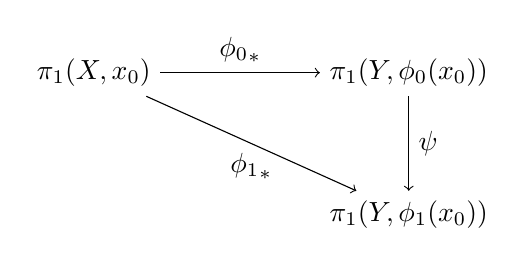
\begin{tikzpicture}[x=1cm, y=0.6cm]
        \node (x0)     at ( 0, 3) {$\pi_1(X, x_0)$};
        \node (phi0x0) at ( 4, 3) {$\pi_1(Y, \phi_0(x_0))$};
        \node (phi1x0) at ( 4, 0) {$\pi_1(Y, \phi_1(x_0))$};
        \draw[->] (x0) -- node [above]{${\phi_0}_*$} (phi0x0);
        \draw[->] (x0) -- node [below]{${\phi_1}_*$} (phi1x0);
        \draw[->] (phi0x0) -- node [right]{$\psi$} (phi1x0);
    \end{tikzpicture} \\
    \end{center}
    換言之,${\phi_1}_*=\psi\circ{\phi_0}_*$。
\end{lemma}
\begin{proof}
    Note that $F(x, 0)=\phi_0(x)$ and $F(x, 1)=\phi_1(x)$ for $x\in X$, so $\lambda$ is a path from $\phi_0(x_0)$ to $\phi_1(x_0)$. \\ 
    By Corollary \ref{path define a isomorphism}, $\psi$ is a isomorphism from $\pi_1(Y, \phi_0(x_0))$ to $\pi_1(Y, \phi_1(x_0))$. \\
    Let $[f]\in\pi_1(X, x_0)$, then $f(0)=x_0$. \\
    Define $H:\textbf{I}\times\textbf{I}\to Y$ by
    \[
        H(x, t) = \begin{cases}
            F(f([1-t]x), 4tx) & x\in[0, \frac{1}{4}], \\
            F(f([1+3t]x-\frac{1}{4}t), t) & x\in[\frac{1}{4}, \frac{1}{2}], \\
            F(f([1-t]x), -2tx+\frac{1}{2}t) & x\in[\frac{1}{2}, 1]. \\
        \end{cases}
    \]
    Since $H(x, 0)=F(f(x), 0)=(\phi_0\circ f)(x)$ and 
    \begin{align*}
        H(x, 1) 
        & = \begin{cases}
            F(f(0), 4x) & x\in[0, \frac{1}{4}], \\
            F(f(4x-\frac{1}{4}), 1) & x\in[\frac{1}{4}, \frac{1}{2}], \\
            F(f(0), 1-(2x-\frac{1}{2})) & x\in[\frac{1}{2}, 1]. \\
        \end{cases} \\
        & = ((\lambda * (\phi_1\circ f)) * \lambda^{-1})(x),
    \end{align*}
    we have $\phi_0\circ f\simeq(\lambda * (\phi_1\circ f)) * \lambda^{-1}$, it follows that $[\phi_0\circ f]=[\lambda * (\phi_1\circ f) * \lambda^{-1}]=\psi([\phi_1\circ f])$ and hence ${\phi_0}_*([f])=(\psi\circ{\phi_1}_*)([f])$. \\
    Therefore, ${\phi_1}_*=\psi\circ{\phi_0}_*$.
\end{proof}

\begin{remark}
    令 $F:\phi_0\simeq\phi_1$ 滿足 $y_0=\phi_0(x_0)=\phi_1(x_0)$:
    \begin{enumerate}
        \item 存在 $[\lambda]\in\pi_1(Y, y_0)$ 使得 $[\phi_0]=[\lambda]{\phi_1}_*[\lambda]^{-1}$。
        \item 若 $\pi_1(Y, y_0)$ 是交換群,則 ${\phi_0}_*={\phi_1}_*$。
    \end{enumerate}
\end{remark}

\begin{theorem}
    令 $\beta:X\to Y$ 為同倫等價,則對於所有 $x_0\in X$,都有 $\beta_*:\pi_1(X, x_0)\to\pi_1(Y, \beta(x_0))$ 為同構。
\end{theorem}
\begin{proof}
    Since $\beta$ is a homotopy equivalence, there is a continuous function $\alpha:Y\to X$ such that $\alpha\circ\beta\simeq 1_X$ and $\beta\circ\alpha\simeq 1_Y$. \\
    By Lemma \ref{homotopy up to pi1 is commutative}, there is a isomorphism $\psi$ such that the lower triangle of the diagram below is commutative; that is, ${1_X}_*=\psi\circ(\alpha\circ\beta)_*$.
    \begin{center}
    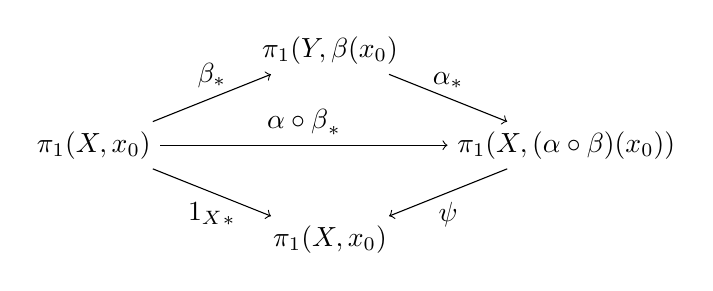
\begin{tikzpicture}[x=1cm, y=0.6cm]
        \node (x0)   at ( 0, 2) {$\pi_1(X, x_0)$};
        \node (abx0) at ( 6, 2) {$\pi_1(X, (\alpha\circ\beta)(x_0))$};
        \node (1x0)  at ( 3, 0) {$\pi_1(X, x_0)$};
        \node (bx0)  at ( 3, 4) {$\pi_1(Y, \beta(x_0)$};
        \draw[->] (x0) -- node [above]{${\alpha\circ\beta}_*$} (abx0);
        \draw[->] (x0) -- node [below]{${1_X}_*$} (1x0);
        \draw[->] (x0) -- node [above]{$\beta_*$} (bx0);
        \draw[->] (abx0) -- node [below]{$\psi$} (1x0);
        \draw[->] (bx0) -- node [above]{$\alpha_*$} (abx0);
    \end{tikzpicture} \\
    \end{center}
    Therefore, $\psi^{-1}=(\alpha\circ\beta)_*$ is a isomorphism. \\
    Since $(\alpha\circ\beta)_*=\alpha_*\circ\beta_*$, so $\beta_*$ is an injective and $\alpha_*$ is a surjective. \\
    Similarly, since $\beta\circ\alpha\simeq 1_Y$, so $\alpha_*$ and $\beta_*$ are bijective. \\
    Hence $\beta_*:\pi_1(X, x_0)\to\pi_1(Y, \beta(x_0))$ is an isomorphism.
\end{proof}

\begin{remark}
    令 $X, Y$ 為路徑連通且有相同倫型的拓樸空間,則對於所有 $x_0\in X$ 和 $y_0\in Y$,都有 $\pi_1(X, x_0)\cong\pi_1(Y, x_0)$。
\end{remark}

\begin{definition}
    令 $X$ 為路徑連通空間。若所有 $x_0\in X$ 滿足 $\pi_1(X, x_0)=\{0\}$,則稱 $X$ 是單連通的 (simply connected)。
\end{definition}

\section{$\pi_1(S^1)$}

\begin{definition}
    令 $f=u+iv:[a, b]\to\mathbb{C}$ 為連續函數,定義積分為
    \[
        \int_a^b f(t) dt = \int_a^b u(t) dt+i\int_a^b v(t) dt.
    \]
\end{definition}

\begin{definition}
    令 $\gamma=x+iy:[a, b]\to\mathbb{C}$ 為函數。若存在 $[a, b]$ 上的有限分割 $P$ 使得 $x, y$ 對 $P$ 的每個區間都是連續可微的,則稱 $\gamma$ 為曲線。 
\end{definition}

\begin{definition}
    令 $\gamma:[a, b]\rightarrow\mathbb{C}$ 為曲線,$f:\gamma([a, b])\to\mathbb{C}$ 為連續函數,則定義 $f$ 沿 $\gamma$ 的積分為
    \[
        \int_\gamma f(z) dz = \int_a^b f(\gamma(t))\gamma'(t) dt,\quad
        \int_\gamma f(z) |dz| = \int_a^b f(\gamma(t))|\gamma'(t)| dt.
    \]
\end{definition}

\begin{definition}
    令 $\gamma:[a, b]\rightarrow\mathbb{C}$ 為閉曲線,$z_0$ 為不在 $\gamma([a, b])$ 上的一點,定義 $\gamma$ 關於 $z_0$ 的卷繞數 (winding number) 為 
    \[
        W(\gamma, z_0) 
        = \frac{1}{2\pi i}\int_\gamma\frac{1}{z-z_0}dz.
    \]
\end{definition}

若 $z_0=0$,則記 $W(\gamma, z_0)$ 為 $W(\gamma)$。 \\

記 $e^{2\pi ix}$ 為 $\exp x$,則 $\frac{d}{dx}\exp x=2\pi i\exp x$。

令 $\gamma:(\textbf{I}, \Dot{\textbf{I}})\to(S^1, 1)$ 為曲線。若函數 $\hat{\gamma}$ 滿足 $\gamma=\exp\circ\ \hat{\gamma}$,則 
\[
    W(\gamma) 
     = \frac{1}{2\pi i}\int_\gamma\frac{1}{z}dz 
     = \frac{1}{2\pi i}\int_0^1\frac{\gamma'(t)}{\gamma(t)}dt 
     = \int_0^1\hat{\gamma}'(t)dt 
     = \hat{\gamma}(1) - \hat{\gamma}(0).
\]

% 須證明
\begin{lemma}
\label{lemma for pi1S1}
    令 $(X, d)$ 為單連通空間,$f:(X, x_0)\to(S^1, 1)$ 為 $\textbf{Top.}$ 的態射,$t_0$ 為整數,並定義 $\exp t=e^{2\pi it}$。存在唯一的態射 $\hat{f}:(X, x_0)\to(\mathbb{R}, t_0)$ 使得 $f=\exp\circ\hat{f}$。
    \begin{center}
    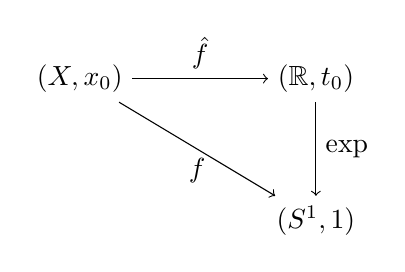
\begin{tikzpicture}[x=1cm, y=0.6cm]
        \node (1) at ( 0, 3) {$(X, x_0)$};
        \node (2) at ( 3, 3) {$(\mathbb{R}, t_0)$};
        \node (3) at ( 3, 0) {$(S^1, 1)$};
        \draw[->] (1) -- node [above]{$\hat{f}$} (2);
        \draw[->] (1) -- node [below]{$f$} (3);
        \draw[->] (2) -- node [right]{$\exp$} (3);
    \end{tikzpicture} \\
    \end{center}
\end{lemma}

\begin{theorem}
    定義 $d:\pi_1(S^1, 1)\to\mathbb{Z}:[f]\mapsto W(f)$,則 $d$ 是同構。
\end{theorem}
\begin{proof}
    Let $[\gamma], [\delta]\in\pi_1(S^1, 1)$, then
    \begin{align*}
        d([\gamma][\delta])
        & = W(\gamma*\delta)
          = \frac{1}{2\pi i}\int_{\gamma*\delta}\frac{1}{z}dz 
          = \frac{1}{2\pi i}\int_\gamma\frac{1}{z}dz +\frac{1}{2\pi i}\int_\delta\frac{1}{z}dz \\
        & = W(\gamma)+W(\delta)
          = d([\gamma])+d([\delta]),
    \end{align*}
    so $d$ is a homomorphism. \\
    Let $m\in\mathbb{Z}$ and set $\gamma:t\to\exp(mt)$, then
    \[
        d([\gamma])
        = W(\gamma)
        = \frac{1}{2\pi i}\int_0^1\frac{\gamma'(t)}{\gamma(t)}dt 
        = m,
    \]
    so $d$ is a surjection. \\
    Let $[\gamma]\in\ker d$, then $W(\gamma)=0$. \\
    By Lemma \ref{lemma for pi1S1}, there exists unique $\hat{\gamma}:(\textbf{I}, \Dot{\textbf{I}})\to(\mathbb{R}, 0)$ such that $\gamma=\exp\circ\hat{\gamma}$. \\
    Then $0=W(\gamma)=\hat{\gamma}(1)-\hat{\gamma}(0)=\hat{\gamma}(1)$. \\
    Since $\hat{\gamma}$ is a loop in $\mathbb{R}$, there is a constant $c$ such that $\hat{\gamma}\simeq c$. \\
    Then $\gamma=\exp\circ\hat{\gamma}\simeq\exp\circ c$, so $[\gamma]=[0]$ and hence $d$ is one-to-one.
\end{proof}

\section{Homology}

\begin{definition}
    令 $\{C_n\}_{n\in\mathbb{Z}}$ 為交換群序列,$\{\partial_n:C_n\to C_{n-1}\}_{n\in\mathbb{Z}}$ 為同態序列。若所有 $n\in\mathbb{Z}$ 滿足 $\im\partial_n\subseteq\ker\partial_{n-1}$,則稱 $(\{C_n\}_{n\in\mathbb{Z}}, \{\partial_n\}_{n\in\mathbb{Z}})$ 為鍊複形 (chain complex),記為 $(C_*, \partial_*)$。
    \begin{center}
    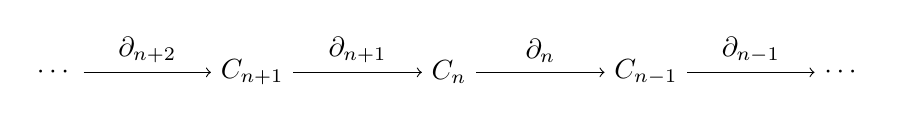
\begin{tikzpicture}[x=2.5cm, y=0.6cm]
        \node (n+2) at (-2, 0) {$\cdots$};
        \node (n+1) at (-1, 0) {$C_{n+1}$};
        \node (n)   at ( 0, 0) {$C_n$};
        \node (n-1) at ( 1, 0) {$C_{n-1}$};
        \node (n-2) at ( 2, 0) {$\cdots$};
        \draw[->] (n+2) -- node [above]{$\partial_{n+2}$} (n+1);
        \draw[->] (n+1) -- node [above]{$\partial_{n+1}$} (n);
        \draw[->] (n) -- node [above]{$\partial_n$} (n-1);
        \draw[->] (n-1) -- node [above]{$\partial_{n-1}$} (n-2);
    \end{tikzpicture} \\
    \end{center}
\end{definition}

$\partial_*$ 稱為 $(C_*, \partial_*)$ 的邊界映射 (boundary map)。

$\im\partial_n\subseteq\ker\partial_{n-1}$ 等價於 $\partial_n\partial_{n-1}=0$。

\begin{definition}
    令 $(C_*, \partial_*)$ 為鍊複形。$\im\partial_{n+1}$ 記為 $B_n(C_*, \partial_*)$,其內元素稱為 $n$-邊界 ($n$-boundaries)。$\ker\partial_n$ 記為 $Z_n(C_*, \partial_*)$,其內元素稱為 $n$-環 ($n$-cycles)。
\end{definition}

$\{C_n\}_{n\in\mathbb{Z}}$ 為交換群序列,因此 $B_n(C_*, \partial_*)$ 和 $Z_n(C_*, \partial_*)$ 皆為正規子群。

\begin{definition}
    令 $(C_*, \partial_*)$ 為鍊複形,則
    \[
        \frac{\ker\partial_n}{\im\partial_{n+1}}
        =
        \frac{Z_n(C_*, \partial_*)}{B_n(C_*, \partial_*)}
    \]
    稱為 $C_*$ 的第 $n$ 階同調群 (homology group),記為 $H_n(C_*)$。
\end{definition}

\section{Singular Homology}

\begin{definition}
    令 $X$ 為拓樸空間,$\sigma:\Delta^n\to X$ 為連續函數,則 $\sigma$ 稱為奇異 $n$-單體 (singular $n$-simplex)。
\end{definition}

由於 $\Delta^1$ 與 $\textbf{I}$ 同胚,因此 $\sigma:\Delta^1\to X$ 可視為 $X$ 中的路徑,而 $\sigma:\Delta^1\to X$ 可視為 $X$ 中的曲面三角形;由此可見,$\sigma:\Delta^n\to X$ 可視為路徑的推廣。

\begin{definition}
    令 $i, n$ 為非負整數。若 $0\le i\le n$,則稱
    \[
        \varepsilon^n_i
        :\Delta^{n-1} \to \Delta^n
        :(t_0, \cdots, t_{n-1}) \mapsto (t_0, \cdots, t_{i-1}, 0, t_i, \cdots, t_{n-1})
    \]
    為面映射 (face map)。
\end{definition}

換言之,$\varepsilon^n_i$ 將 $\Delta^{n-1}$ 映到 $\Delta^n$ 邊界上位於 $e^i$ 對面的 $(n-1)$-面。

$\sigma$ 和 $\varepsilon^n_i$ 複合形成的奇異 $(n-1)$-單體 $\sigma\circ\varepsilon^n_i:\Delta^{n-1}\to X$ 即可用於討論 $\Delta^n$ 邊界上的其中一個 $(n-1)$-面。

\begin{lemma}
\label{Commutative of face map}
    若 $0\le i<j\le n$,則 $\varepsilon^{n+1}_j\circ\varepsilon^n_i=\varepsilon^{n+1}_i\circ\varepsilon^n_{j-1}$。
\end{lemma}
\begin{proof}\begin{align*}
        (\varepsilon^{n+1}_j\circ\varepsilon^n_i)(t_0, \cdots, t_{n-1}) 
        & = (t_0, \cdots, t_{i-1}, 0, t_i, \cdots, t_j, 0, t_{j-1}, \cdots, t_n) \\
        & = (\varepsilon^{n+1}_i\circ\varepsilon^n_{j-1})(t_0, \cdots, t_{n-1}).
\end{align*}
\end{proof}

如同路徑複合 $f*g$ 和反路徑 $f^{-1}$ 定義了基本群,透過自由交換群的運算與定向單體的奇偶性可以定義奇異 $n$-單體上的同調群。

\begin{definition}
    令 $n$ 為正整數,$[e_{i_0}, \cdots, e_{i_n}], [e_{j_0}, \cdots, e_{j_n}]$ 為定向 $n$-單體。若 $[e_{i_0}, \cdots, e_{i_n}]$ 和 $[e_{j_0}, \cdots, e_{j_n}]$ 的置換 
    \[
        \begin{bmatrix}
            0 & 1 & \cdots & n \\
            e_{i_0} & e_{i_1} & \cdots & e_{i_n}
        \end{bmatrix},
        \begin{bmatrix}
            0 & 1 & \cdots & n \\
            e_{j_0} & e_{j_1} & \cdots & e_{j_n}
        \end{bmatrix}
    \]
    有相同的奇偶性,則稱兩者方向相同,記為 $[e_{i_0}, \cdots, e_{i_n}] = [e_{j_0}, \cdots, e_{j_n}]$;否則稱兩者方向相反,記為 $[e_{i_0}, \cdots, e_{i_n}]=-[e_{j_0}, \cdots, e_{j_n}]$。
\end{definition}

例如 $[e_0, e_1]=-[e_1, e_0]$ 及 $[e_0, e_1, e_2]=[e_1, e_2, e_0]=-[e_1, e_0, e_2]$。

$\Delta^0$ 則視 $[e_{i_0}]=-[e_{i_0}]$。 \\

舉例來說,定向 $1$-單體的奇偶性可視為路徑的正反定向,而定向 $2$-單體的奇偶性可視為三角形上的順時針或逆時針定向。

\begin{definition}
    令 $X$ 為拓樸空間,$n$ 為整數。若 $n\ge0$,令 $S_n(X)$ 為 $\{\sigma\ |\ \sigma\text{ 為奇異 }n\text{-單體}\}$ 生成的自由交換群;若 $n<0$,令 $S_n(X)$ 為平凡群。稱 $S_n(X)$ 為 $n$-鍊 ($n$-chain)。
\end{definition}

$\sigma_1+\sigma_2$ 可視為 $\sigma_1$ 和 $\sigma_2$ 的疊加圖形,$-\sigma$ 可視為在奇偶性上反向定義的 $\sigma$,如同不要求首尾相接且無視複合順序的路徑複合運算。

以路徑 $f$ 為例,$f+f=2f$ 相當於沿著 $f$ 路徑走兩次。 \\

奇異 $n$-單體的邊界是奇異 $(n-1)$-單體的疊加圖形,視如同 $\partial\sigma\in S_{n-1}(X)$,因此邊界映射可以由 $\sigma\circ\varepsilon^n_i$ 的疊加構成。 \\

考慮由曲面三角形 $\sigma_i:\Delta^2\to\mathbb{R}^3$ 拼接而成的球殼 $\sum_i\sigma_i\in S_2(X)$。

球殼的邊界則由線段 $\sigma_j:\Delta^1\to\mathbb{R}^3$ 疊加而成。

若所有曲面三角形皆以逆時針定向,則三角形之間的邊界可以相互消去。

換言之,$\partial\left(\sum_i\sigma_i\right)=0$,而由此可見,$\ker\partial$ 內的元素可視為封閉圖形。 \\

然而,若邊界映射由 $\sigma\circ\varepsilon^n_i$ 的疊加構成,則封閉路徑有可能不落於 $\ker\partial$。

因此我們在邊界上進一步的考慮奇偶性,同時使得圖形的邊界皆可由封閉圖形表達;換言之,$\im\partial_n\subseteq\ker\partial_{n+1}$。 \\

封閉路徑的邊界可視為 $\sigma\circ\varepsilon^1_0$ 和 $\sigma\circ\varepsilon^1_0$,並且滿足 $\sigma\circ\varepsilon^1_0-\sigma\circ\varepsilon^1_0=0$。

而定向 $2$-單體 $[e_0, e_1, e_2]$ 的邊界可視為封閉圖形 $[e_0, e_1]-[e_0, e_2]+[e_1, e_2]$。

由此可知,邊界映射應由 $(-1)^i (\sigma\circ\varepsilon^n_i)$ 的疊加構成。

\begin{definition}
    令 $X$ 為拓樸空間,$n$ 為整數。若 $n>0$,令 $\partial_n:S_n(X)\to S_{n-1}(X)$ 為同態且滿足 $\partial_n\sigma=\sum_{i=0}^n (-1)^i (\sigma\circ\varepsilon^n_i)$;若 $n\le0$,令 $\partial_n\sigma=0$。稱 $\partial_n$ 為邊界算子 (boundary operator)。
\end{definition}

\begin{remark}
\label{property of boundary operator}
    令 $\sum_i n_i \sigma_i\in S_n(X)$,則 $\partial_n\left(\sum_i n_i \sigma_i\right)=\sum_i n_i \partial_n(\sigma_i)$。 
\end{remark}

\begin{theorem}
    $\partial_n\partial_{n+1}=0$。
\end{theorem}
\begin{proof}
    Let $\sigma$ be a singular $(n+1)$-simplex. \\
    Set $\hat{i}=j$ and $\hat{j}=i-1$, then by Lemma \ref{Commutative of face map},
    \begin{align*}
        \partial_n\partial_{n+1}\sigma
        & = \sum_j(-1)^j\left(\sum_i(-1)^i\sigma\circ\varepsilon^{n+1}_i\right)\circ\varepsilon^n_j \\
        & = \sum_{i\le j}(-1)^{i+j}\sigma\circ\varepsilon^{n+1}_i\circ\varepsilon^n_j+\sum_{i>j}(-1)^{i+j}\sigma\circ\varepsilon^{n+1}_i\circ\varepsilon^n_j \\
        & = \sum_{i\le j}(-1)^{i+j}\sigma\circ\varepsilon^{n+1}_i\circ\varepsilon^n_j+\sum_{\hat{i}\le\hat{j}}(-1)^{\hat{i}+\hat{j}+1}\sigma\circ\varepsilon^{n+1}_{\hat{i}}\circ\varepsilon^n_{\hat{j}} 
        = 0.
    \end{align*}
    Let $\sum_k n_k \sigma_k\in S_n(X)$, then by Remark \ref{property of boundary operator}, $\partial_n\partial_{n+1}\left(\sum_k n_k \sigma_k\right)=0$. \\
\end{proof}

\begin{definition}
    令 $X$ 為拓樸空間。稱 $(S_*(X), \partial_*)$ 為奇異鍊複形 (singular complex),$n$-邊界 $\im\partial_{n+1}=B_n(S_*(X), \partial_*)$ 記為 $B_n(X)$,$n$-環 $\ker\partial_n=Z_n(S_*(X), \partial_*)$ 記為 $Z_n(X)$。
\end{definition}

\begin{definition}
    令 $(S_*(X), \partial_*)$ 為奇異鍊複形。稱 $H_n(S_*(X))$ 為奇異同調群 (singular homology group),記為 $H_n(X)$。
\end{definition}

接著證明 $H_n$ 是函子。

\begin{definition}
    令 $f:X\to Y$ 為連續函數。定義 $f_\#$ 為由 $S_n(X)$ 到 $S_n(Y)$ 的同態,且所有奇異 $n$-單體 $\sigma$ 滿足 $f_\#(\sigma)=f\circ\sigma$。
\end{definition}

\begin{remark}
    令 $\sum_i n_i \sigma_i\in S_n(X)$,則 $f_\#\left(\sum_i n_i \sigma_i\right)=\sum_i n_i f_\#(\sigma_i)$。 
\end{remark}

\begin{lemma}
    令 $f:X\to Y$ 為連續函數,則 $\partial_n\circ f_\#=f_\#\circ \partial_n$。
    \begin{center}
    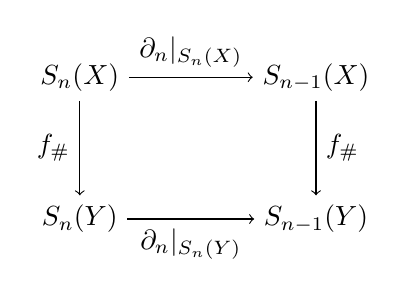
\begin{tikzpicture}[x=1cm, y=0.6cm]
        \node (SnX)   at ( 0, 3) {$S_n(X)$};
        \node (SnY)   at ( 0, 0) {$S_n(Y)$};
        \node (Sn-1X) at ( 3, 3) {$S_{n-1}(X)$};
        \node (Sn-1Y) at ( 3, 0) {$S_{n-1}(Y)$};
        \draw[->] (SnX) -- node [above]{$\partial_n|_{S_n(X)}$} (Sn-1X);
        \draw[->] (SnY) -- node [below]{$\partial_n|_{S_n(Y)}$} (Sn-1Y);
        \draw[->] (SnX) -- node [left]{$f_\#$} (SnY);
        \draw[->] (Sn-1X) -- node [right]{$f_\#$} (Sn-1Y);
    \end{tikzpicture} \\
    \end{center}
\end{lemma}
\begin{proof}
    Let $\sigma:\Delta^n\to X$ be a singular $n$-simplex, then
    \[
        (f_\#\circ\partial_n)(\sigma)
         = f_\#\left(\sum_{i=0}^n(-1)^i(\sigma\circ\varepsilon^n_i)\right)
          = \sum_{i=0}^n(-1)^i(f\circ\sigma\circ\varepsilon^n_i)
         = (\partial_n\circ f_\#)(\sigma).
    \]
\end{proof}

\begin{lemma}
    令 $f:X\to Y$ 為連續函數,則 $f_\#(Z_n(X))\subseteq Z_n(Y)$ 且 $f_\#(B_n(X))\subseteq B_n(Y)$。
\end{lemma}
\begin{proof}
    Let $\alpha\in Z_n(X)$, then $\partial_n(\alpha)=0$ and hence 
    \[
        (\partial_n\circ f_\#)(\alpha)=(f_\#\circ\partial_n)(\alpha)=f_\#(0)=0.
    \]
   Let $\beta\in B_n(X)$, then $\partial_{n+1}(\gamma)=\beta$ for some $\gamma\in S_{n+1}(X)$. \\
   It follows that $f_\#(\beta)=(f_\#\circ\partial_{n+1})(\gamma)=(\partial_{n+1}\circ f_\#)(\gamma)\in B_n(Y)$.
\end{proof}

\begin{theorem}
    $H_n:\textbf{Top}\to\textbf{Ab}$ 是函子。
\end{theorem}
\begin{proof}
    Note that $H_n(X)$ is abelian if $X$ is a topological space. \\
    Let $f:X\to Y$ be a continuous function, define 
    \[
        H_n(f):H_n(X)\to H_n(Y):z_n+B_n(X)\mapsto f_\#(z_n)+B_n(Y),
    \]
    where $z_n\in Z_n(X)$. \\
    Let $x_n, y_n\in Z_n(X)$. \\ 
    If $x_n+B_n(X)=y_n+B_n(X)$, then $x_n-y_n\in B_n(X)$ \\
    Since $f_\#(B_n(X))\subseteq B_n(Y)$, we have
    \begin{align*}
        H_n(f)(x_n+B_n(X))
        & = f_\#(x_n)-f_\#(y_n)+f_\#(y_n)+B_n(Y) \\
        & = H_n(f)(y_n+B_n(X)).
    \end{align*}
    Therefore, $H_n$ is well-define. \\
    Since $f_\#$ is a homomorphism, so $H_n(f)$ is a homomorphism. \\
    Let $g:Y\to Z$ be a continuous function, then $H_n(g\circ f)(x_n+B_n(X))=g\circ f\circ x_n+B_n(Y)=(H_n(g)\circ H_n(f))(x_n+B_n(X))$. \\
    Since $(H_n(f)\circ H_n(1_X))(x_n+B_n(X))=H_n(f)(x_z+B_n(X))$, we conclude that $H_n$ is a functor.
\end{proof}

\begin{corollary}
    若 $X, Y$ 同胚,則 $H_n(X)\cong H_n(Y)$。
\end{corollary}
\begin{proof}
    Suppose that $f:X\to Y$ is the homeomorphism, then $f^{-1}\circ f=1_X$. \\
    Since $H_n(f^{-1}\circ f)=H_n(f^{-1})\circ H_n(f)=H_n(1_X)=1_{H_n(X)}$
\end{proof}

\begin{remark}
    $S_n:\textbf{Top}\to\textbf{Ab}$ 是函子。
\end{remark}
\begin{proof}
    Define $S_n:f\mapsto f_\#$, then $S_n(f)$ is a homomorphism. \\
    Let $f:X\to Y, g:Y\to Z$ be continuous functions and $\sigma:\Delta^n\to X$ be a singular $n$-simplex, we have $S_n(g\circ f)(\sigma)=g\circ f\circ\sigma=[S_n(g)\circ S_n(f)](\sigma)$ and $S_n(f\circ 1_X)(\sigma)=f\circ 1_X\circ\sigma=[S_n(f)\circ S_n(1_X)](\sigma)$, so $S_n(X)$ is a functor.
\end{proof}

接著討論 singular homology 的性質。

\begin{theorem}[Dimension Axiom]
    若 $X$ 為單元素集合,則$H_n(X)=0$ 對於所有 $n>0$。
\end{theorem}
\begin{proof}
    Suppose that $X=\{x_0\}$, then $S_n(X)=\<\sigma_n:\Delta^n\to X:x\mapsto x_0\>$. \\
    Let $m\sigma_n\in S_n(X)$, where $m\in\mathbb{Z}$, then
    \[
        \partial_n m\sigma_n 
        = m\sum_{i=0}^n(-1)^i\sigma_n\circ\varepsilon_i
        = \left(m\sum_{i=0}^n(-1)^i\right)\sigma_{n-1}
        = \begin{cases}
            0 & n \text{ is odd} \\
            m\sigma_{n-1} & n \text{ is even}
        \end{cases}.
    \]
    If $n$ is odd, then $Z_n(X)=\ker\partial_n=S_n(X)$. \\
    Since $\partial_{n+1}m\sigma_{n+1}=m\sigma_n$ for $m\sigma_n\in S_n(X)$, so $B_n(X)=\im\partial_{n+1}=S_n(X)$. \\
    Therefore, $H_n(X)=Z_n(X)/B_n(X)=0$. \\
    Otherwise, $Z_n(X)=\ker\partial_n=0$ and hence $\partial_n$ is a bijection. \\
    It follows that $H_n(X)=Z_n(X)/B_n(X)=0$.
\end{proof}

\begin{lemma}
    若 $X$ 是路徑連通空間,則 $H_0(X)\cong\mathbb{Z}$。
\end{lemma}
\begin{proof}
    For each $x_0\in X$, define a singular $0$-simplex $\sigma_{x_0}:x\mapsto x_0$. \\
    Let $x, y\in X$, there is a path $\gamma$ from $x$ to $y$. \\
    Define $\sigma_\gamma:\Delta^1\to X:te_0+(1-t)e_1\mapsto \gamma(1-t)$. \\
    Then $\partial_1\sigma_\gamma=\sigma_\gamma\circ\varepsilon_0^1-\sigma_\gamma\circ\varepsilon_1^1=\sigma_y-\sigma_x\in\im\partial_1=B_0(X)$. \\
    Therefore, $\sigma_x+B_0(X)=\sigma_y+B_0(X)$ for all $y\in X$. \\
    Let $\sum n_i\sigma_{x_i}\in S_0(X)$, note that $Z_0(X)=S_0(X)$. \\
    Since $B_0(X)$ is normal, 
    \[
        \left(\sum_i n_i\sigma_{x_i}\right)+B_0(X)
        = \sum_i n_i(\sigma_{x_i}+B_0(X))
        = \left(\sum_i n_i\right)(\sigma_x+B_0(X)).
    \]
    Hence $H_0(X)$ is a cyclic group generated by $\sigma_x+B_0(X)$.
\end{proof}

\begin{theorem}
    若 $\{X_\lambda\ |\ \lambda\in\Lambda\}$ 為連通單元的蒐集且 $X=\bigcup_{\lambda\in\Lambda}X_\lambda$,則 $H_n(X)\cong\prod_{\lambda\in\Lambda}H_n(X_\lambda)$。
\end{theorem}
\begin{proof}
    Note that $\sigma$ is singular $n$-simplex implies $\im\sigma\subseteq X_\lambda$ for some $\lambda\in\Lambda$. \\
    For each $\sigma=\sum_i n_i\sigma_i\in S_n(X)$ and $\lambda\in\Lambda$, define $\sigma_\lambda=\sum_j n_{i_j}\sigma_{i_j}$ where $\sigma_{i_j}:\Delta^n\to X_\lambda$, then $\sigma_\lambda\in S_n(X_\lambda)$ and $\sigma=\sum_{\lambda\in\Lambda}\sigma_\lambda$. \\
    For each $n$, define
    \[
        \theta_n:H_n(X)\to\prod_{\lambda\in\Lambda}H_n(X_\lambda):\sigma+B_n(X)\mapsto(\sigma_\lambda+B_n(X_\lambda))_{\lambda\in\Lambda}.
    \]
\end{proof}

\end{CJK}
\end{document}
